\documentclass[areasetadvanced]{scrartcl}

\usepackage[utf8]{inputenc}
\usepackage[T2A]{fontenc}

\usepackage{graphicx}
\usepackage{url}

\usepackage[footskip=1cm,left=25mm, right=15mm, top=20mm, bottom=20mm]{geometry}
\usepackage{setspace}
\usepackage{booktabs}
\usepackage{multirow}
\usepackage{amsmath, amssymb}
\usepackage{graphicx}
\usepackage{tikz}
\usetikzlibrary{arrows.meta}
\usepackage{float}
\usepackage{caption}
\DeclareCaptionLabelSeparator{dash}{ - }
\captionsetup{labelsep=dash}
\captionsetup[figure]{name={Рис.}}
\captionsetup[table]{name={Таблица}, position=top, justification=raggedleft, singlelinecheck=false}
\usepackage{dashrule}
\usepackage{fancyhdr}
\usepackage{hyperref}
\usepackage{parskip}
\usepackage{textcomp, enumitem}
\usepackage{indentfirst}
\usepackage{graphicx}
\usepackage{algorithm}
\usepackage{pdfpages}
\usepackage{algpseudocode}
\usepackage{array}
\newcolumntype{R}[1]{>{\raggedright\arraybackslash}m{#1}}
\usepackage{geometry}
\usepackage{afterpage}
\usepackage{minted}
\usepackage{adjustbox}
\setcounter{secnumdepth}{3}
\setcounter{tocdepth}{3}
\usepackage{listings}

\tikzstyle{block} = [rectangle, rounded corners, minimum width=3cm, minimum height=1cm, text centered, draw=black, fill=lightgray]

\setkomafont{sectioning}{\normalfont\bfseries}
\setkomafont{section}{\normalfont\Large\bfseries}
\setkomafont{subsection}{\normalfont\large\bfseries}
\setkomafont{subsubsection}{\normalfont\large\bfseries}
\setkomafont{paragraph}{\normalfont\large\bfseries}

\lstset{
  language=Haskell,
  basicstyle=\ttfamily\small,
  keywordstyle=\color{blue}\bfseries,
  stringstyle=\color{red},
  commentstyle=\color{green!70!black},
  numbers=left,
  numberstyle=\tiny,
  stepnumber=1,
  numbersep=10pt,
  showstringspaces=false,
  breaklines=true,
  frame=single
}

\setcounter{tocdepth}{2}
\begin{document}
\sloppy
	\thispagestyle{empty}
	\begin{center}
		\large{МИНОБРНАУКИ РОССИИ} \par
		\vspace{0.3cm}
		\normalsize
		{ФЕДЕРАЛЬНОЕ ГОСУДАРСТВЕННОЕ АВТОНОМНОЕ ОБРАЗОВАТЕЛЬНОЕ УЧРЕЖДЕНИЕ ВЫСШЕГО ОБРАЗОВАНИЯ} \par
		\vspace{0.3cm}
		\textbf{\guillemotleft САНКТ-ПЕТЕРБУРГСКИЙ ПОЛИТЕХНИЧЕСКИЙ}
		\textbf{УНИВЕРСИТЕТ ПЕТРА ВЕЛИКОГО\guillemotright} \par
		\vspace{0.3cm}
		{Институт компьютерных наук и кибербезопасности}\par
		{Высшая школа технологий искусственного интеллекта}\par
	\end{center}
	\vfill
	\begin{center}
		{\large Отчет по дисциплине \guillemotleft ЦИФРОВЫЕ РЕСУРСЫ В НАУЧНОМ ИССЛЕДОВАНИИ\guillemotright}\par
		
		 Обзор литературы \par
            {\huge \guillemotleft Линеаризация механизма внимания в трансформерных сегментаторах\guillemotright}
         
	\end{center}
	\vfill
	\begin{flushleft}
		Студент: \hspace{1.8cm} \rule[0pt]{2.5cm}{0.5pt}\hfill Салимли А. М.\par
		\vspace{1.5cm}
		Преподаватель: \hspace{0.55cm} \rule[0pt]{2.5cm}{0.5pt}\hfill  Моторин Д. Е.
	\end{flushleft}
	\vspace{0.5cm}
	\begin{flushright}
		\guillemotleft \rule[0pt]{0.8cm}{0.5pt}\guillemotright \rule[0pt]{2cm}{0.5pt} 20\rule[0pt]{0.5cm}{0.5pt} г.
	\end{flushright}
	\vfill
	\begin{center}
		Санкт-Петербург, 2026г.
	\end{center}
	\newpage
	\tableofcontents
	\newpage
\section*{Введение}
	\addcontentsline{toc}{section}{Введение}
	Появление механизма внимания и трансформеров, изначально предложенных для задач обработки 
	естественного языка, привело к их последующей интеграции в задачи компьютерного зрения, в том числе для задач 
	семантической и экземплярной сегментации. Ключевым преимуществом таких моделей является способность
	моделировать глобальные и локальные зависимости между удаленными областями изображения уже
	на ранних стадиях обработки тогда как в сверточных архитектурах глобальный
	контекст формируется лишь с помощью последовательных операций сверток.

	Ограничение сверточных архитектур видно при попытке сегментировать мелкогабаритные или тонкие протяженные объекты, такие как
	ЖД и трамвайные рельсы, так как они занимают малую долю площади всего кадра и имеют изменчивую ширину и длину на кадрах \cite{myarticle}. Помимо этого, 
	их признаки существенно изменяются из-за искожений кадра, бликов, теней и окклюзий, в последствии чего, энкодер CNN приводит к утрате информации, из-за 
	чего маски сегмента могут получится либо оборванными либо не накладываться вообще. 
	Экземплярная сегментация так же не решает такую проблему. Например сети унаследывавшие принципт YOLACT, которые используют наложение итоговой маски как линейную 
	комбинацию прототипных карт с последующим обрезанием по ограничивающей рамки так же не справляются с моментами когда тень падает на рельсы или на кадрах есть блики. 
	Помимо этого ограничивающая рамка может обрезать кусок маски сегмента если ветка детекции не уловит рельсы целеком \cite{myarticle}. 

	С внедрением архитектур на основе Vision Transformer (ViT), точность сегментации для тонких и мелкогабаритных объектов заметно выросла, что обусловило 
	применение трансформерных сегментаторов и детекторов в задачах компьютерного зрения. 

	В рамках выпускной квалификационной работы и исследования решалась задача обучения и сравнительного анализа моделей сегментации трамвайных рельс с последующем построением 
	динамической зоны интереса, детекции и трекинга посторонних объектов. Были обучены и сравнены следующие сегментаторы: 
	\begin{itemize}
		\item DeepLabV3+ с остаточной сетью энкодером ResNet (50, 101);
		\item YOLO-seg (8n, 8s, 11s, 26s);
		\item SegFormer B0.
	\end{itemize}

	Результаты проведенных обучений, валидаций и тестов показали что классические сверточные сети демонтрируют хоть и хорошое но не идеальное качество по средним метрикам IoU и Dice.
	
	Модель SegFormer \cite{segformer}, построенная на механизме эффективного самовнимания
	(Efficient Self-Attention, ESA), была представлена в эксперименте наименьшей c конфигурацией
	B0, содержащей приблизительно 3.8 млн обучаемых параметров. Несмотря на столь
	малое число параметров, данная модель показала конкурентоспособные значения
	метрик качества. Это позволяет предположить, что переход к более емким конфигурациям семейства B3 и B5 обеспечил бы прирост mIoU и mDice, 
	заметно превосходящий показатели рассмотренных сверточных архитектур.

	Однако модель не была выбрана в веду того, что используемый в SegFormer механизм ESA имеет сложность $O(\frac{N^2}{R})$, где $N$ - число пикселей, а $R$ - коэффициент понижения размерности.

	Вся проблема заключается в квадратичной сложности, что дает сильное ограничение на скорость инференса и обучение модели.
	В литературе активно развивается направление линеаризации механизма внимания. Целью таких исследований является снижение асимптотической сложности до $O(N)$,
	при сохранении способности моделировать глобальные зависимости. Отсюда следует гипотеза исследования для магистерской диссертации - линеаризация механизма внимания в архитектуре 
	SegFormer позволяющая получить сегментатор сочитающий быструю скорость инференса сравнимую для работы в реальном времени и сохраняющую точность свойственную трансформерной архитектре.
	
	Ниже представлен обзор работ по линеаризации механизма внимания в сегментаторах.
	Сначала сравниваются постановки задач и то что авторы считают проблемой. Потом разбираются сами методы снижения сложности внимания и то
	куда его вставляют в сети. После этого сравниваются экспериментальные результаты по точности и по скорости. Отдельно собрано то что
	в работах говорится про тонкие протяженные объекты, так как именно они интересны для сегментации рельсов. Сведения о журналах и авторах
	рассмотренных статей приведены в приложении А.

	\newpage
	\section{Обзор литературы}
	\subsection{Постановки задач}
		Во всех рассмотренных статьях решается одна и таже основная задача - линеаризация 
		механизма внимания в сегментаторах типа ViT. Каждому пикселю нужно присвоить класс а сеть должна видеть
		соседние пиксели и дальний контекст (т.е как выбранный пиксель связан с дальними). 
		Различаются работы данными и тем какие требования считаются главными.

		Первая группа это сегментация сцен общего характера (на датасетах типа городской среды). Сюда входят SegFormer \cite{segformer}, LSNet \cite{lsnet}, RTLinearFormer \cite{rtlinearformer}
		и HLSM-ViT \cite{hlsmvit}. Данные тут публичные - в основном это датасеты city scapes, camvid, ADE20K и COCO-stuff и главное требование это
		скорость инференса при высоком разрешении кадра. Постановка проблемы у них разная. В SegFormer \cite{segformer} авторы говорят про архитектуру
		целиком, так как обычный ViT делает признаки только одного масштаба и слишком вычислительно-сложный на больших изображениях к тому же аналоговые модели типа PVT, 
		Swin и Twins улучшили только кодировщик
		и оставили тяжелый декодировщик. В LSNet \cite{lsnet} узким местом названо само внимание потому что требует слишком много памяти
		и времени из-за чего в быстрых сетях внимание обычно вообще не ставят, а в облегченных вариантах отказываются от попарных связей между
		пикселями и теряют границы сегментаии. В RTLinearFormer \cite{rtlinearformer} проблема сформулирована так что двухразрешающие сети остаются
		полностью сверточными именно потому что квадратичное внимание на ветви высокого разрешения слишком дорогое. В статье про архитектуру HLSM-ViT \cite{hlsmvit} исходят из 
		того что линейная сложность уже
		 сделана и говорят что проблема это ее последствия. Карта внимания после линеаризации
		размывается а ее ранг падает, у авторов он равен 71 при полном ранге 128.
		Конкретного прикладного объекта в этой группе нет - задача сводится к самой линеаризации внимания и сравнению моделей на открытых датасетах,
		где сразу размечены десятки классов городской сцены. Немного в стороне стоит HLSM-ViT \cite{hlsmvit}, где линейное внимание проверяют как
		универсальный костяк - сначала на классификации, потом на детекции и только затем на сегментации сцен.

		Вторая группа это уже снимки с воздуха и большая часть промышленные изображения. В статьях про архитектуру GLANet \cite{glanet} и ABCFNet \cite{abcfnet} работают с
		воздушными фото и спутниковыми снимками, в LPT-Net \cite{lptnet} с углем на конвейере, CA-UNet \cite{caunet} с микроструктурой
		сплавов MS-LCFNet \cite{mslcfnet} с листьями томатов, а FESS-SAM \cite{fesssam} со снимками тоннелей метро. Данные тут чаще собраны самими
		авторами объекты плохо отделяются от фона и сильно различаются по масштабу. В GLANet \cite{glanet} сказано что скалярное внимание при
		большом разрешении неприменимо а разреженные и хеширующие приближения не дают нужного баланса скорости и качества. В ABCFNet \cite{abcfnet}
		добавлена вторая проблема - при многократном понижении разрешения теряются границы и мелкие объекты а Swin и ViT хоть и дают контекст
		но квадратичны и не связывают пространственное измерение с канальным. LPT-Net \cite{lptnet} и CA-UNet \cite{caunet} ставят задачу как работу в
		реальном времени на производстве. У LPT-Net - 95.7 FPS а у CA-UNet около 6 изображений в секунду.
		В статье с архитектурой MS-LCFNet \cite{mslcfnet} главной проблемой считают слабую семантику одного снимка и добавляют к изображению
		текстовое описание эксперта а сложность внимания идет вторым вопросом. FESS-SAM \cite{fesssam} интересен как противоположный случай. Авторы
		вообще не занимаются линеаризацией - сегментацию делает предобученная SAM с полным
		квадратичным вниманием. Эта работа нужна в обзоре так как может быть сегментаторы SAM смогут сегментировать тонкие объекты.
		По тому что именно надо выделить группа тоже распадается. В GLANet \cite{glanet} и ABCFNet \cite{abcfnet} размечают земной покров -
		застроенные и непроницаемые поверхности, здания, низкую растительность, деревья и автомобили, причем ABCFNet дополнительно проверяют на дорогах
		и полях снимков DeepGlobe. LPT-Net \cite{lptnet} отделяет куски пустой породы от угля в потоке на конвейерной ленте, CA-UNet \cite{caunet}
		выделяет включения второй фазы на снимке микроструктуры сплава, а MS-LCFNet \cite{mslcfnet} - пятна пяти болезней на листе томата.
		FESS-SAM \cite{fesssam} ближе всех по типу объекта к рельсам, так как там размечают сразу все элементы стены тоннеля - светлые и темные кабели,
		контактный провод, пожарный и металлический трубопроводы, эвакуационную платформу и болтовые отверстия, то есть длинные тонкие линии,
		протянутые через весь кадр.

		Третья группа это медицинские изображения. Сюда входят MLFormer \cite{mlformer}, MASA-VMUNet \cite{masavmunet},
		WTP-MILA-UNet \cite{wtpmilaunet}, CLT-MambaSeg \cite{cltmambaseg}, Snake-RWKV \cite{snakerwkv}, UUEKAN \cite{uuekan} и работа по брюшной полости \cite{pmp} (PMP). 
		Модальности разные - КТ, МРТ, УЗИ и рентгеновские снимки, но постановка
		проблемы почти одинаковая. Сверточные U-Net не видят дальних зависимостей и трансформеры квадратичны и плохо учатся на малых выборках а модели
		пространства состояний дают линейную сложность но хуже сегментируют мелкие детали и границы. Дальше начинаются отличия. В WTP-MILA-UNet \cite{wtpmilaunet}
		главная сложность это крошечная выборка всего 18 пациентов и из-за этого модель переносят с других датасетов. В CLT-MambaSeg \cite{cltmambaseg}
		нехватку данных решают генеративной аугментацией. В PMP \cite{pmp} задача осложнена тем что проблемы рассеяны по всей брюшной полости и границы
		у них размытые а вычисления ограничены оборудованием больницы. Snake-RWKV \cite{snakerwkv} формулирует проблему которой нет у остальных.
		При развертке двумерной карты признаков в одномерную последовательность соседние пиксели тонкого сосуда расходятся далеко друг от друга. 
		В статье про сеть UUEKAN \cite{uuekan} тоже смотрят на недостатки линейного внимания и говорят про
		слишком сглаженное распределение весов то есть повторяет проблему сети HLSM-ViT \cite{hlsmvit} но уже в медицинской задаче.
		Цели сегментации внутри группы тоже разные. В MLFormer \cite{mlformer}, MASA-VMUNet \cite{masavmunet}, CLT-MambaSeg \cite{cltmambaseg} и
		UUEKAN \cite{uuekan} одного конкретного объекта нет - линейное внимание сравнивают на открытых наборах, где размечены органы брюшной полости,
		отделы сердца и очаги поражения на снимках кожи, УЗИ и эндоскопии. В WTP-MILA-UNet \cite{wtpmilaunet} выделяют печень на МРТ, в
		Snake-RWKV \cite{snakerwkv} - тонкие ветвящиеся сосуды сердца на рентгеновских снимках, а в PMP \cite{pmp} - рассеянные по брюшной полости
		очаги на КТ.

		Требования к эффективности у этих трех групп разные. В сегментации сцен эффективность меряют кадрами в секунду на полном разрешении,
		в снимках ДЗЗ и промышленных задачах чаще памятью и FLOPs, а в медицине обычно числом параметров и FLOPs, при этом реальная задержка приводится
		только в MLFormer \cite{mlformer}, Snake-RWKV \cite{snakerwkv} и UUEKAN \cite{uuekan}. Из-за этого эффективность в разных
		статьях означает разные вещи. 

	\subsection{Способы линеаризации}
		Если смотреть только на сами механизмы линеаризации то все статьи можно разлажить на пять семейств.

		Первое это понижение размерности ключей и значений при сохранении softmax. Так устроен механизм ESA в SegFormer \cite{segformer}
		(см. рис. \ref{segformerarch}). Ключи и значения сжимаются в $R$ раз и сложность падает до $O(N^2/R)$, но она остается квадратичной по числу
		пикселей и выигрыш от $R$.

		\begin{figure}[H]
			\center
			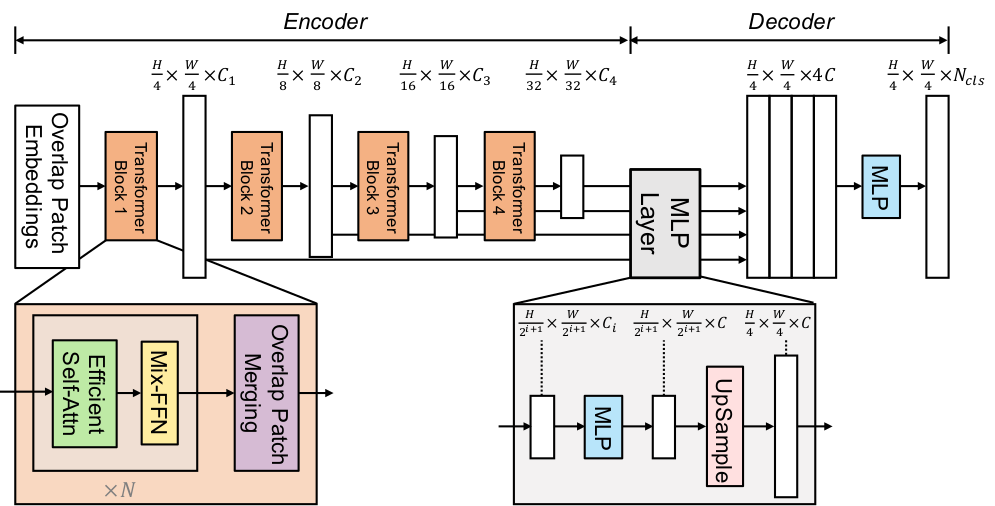
\includegraphics[width=0.5\linewidth]{img/SEGFROMER_ARCH.png}
			\caption{Архитектура SegFormer \cite{segformer}}
			\label{segformerarch}
		\end{figure}

		Тот же прием встречается и в медицинских работах. В MLFormer \cite{mlformer}
		 между кодировщиком и декодировщиком собран именно на таком внимании с коэффициентами сжатия от 1 до 8 по стадиям, то есть авторы линеаризуют
		основные блоки но в месте сети для точности сегментации оставляют механизм из SegFormer.


		Второе преимущественное это ядерное линейное внимание. Идея у всех такая что - softmax заменяется произведением неотрицательных функций
		от запросов и ключей и потом порядок умножения матриц меняется - сначала считается матрица размера $d \times d$
		$$O_i = \frac{\phi(Q_i) \sum_{j=1}^{N} \phi(K_j)^T V_j}{\phi(Q_i) \sum_{j=1}^{N} \phi(K_j)^T}$$
		Сложность после этого линейна по числу пикселей. Отличаются работы выбором ядра $\phi$ и тем чем компенсируют потерю.
		В LSNet \cite{lsnet} ядром служит ReLU, а перед ним запросы и ключи проходят свертку и блок Disentangled Non-Local
		(см. рис. \ref{lsnetattn}).

		\begin{figure}[H]
			\center
			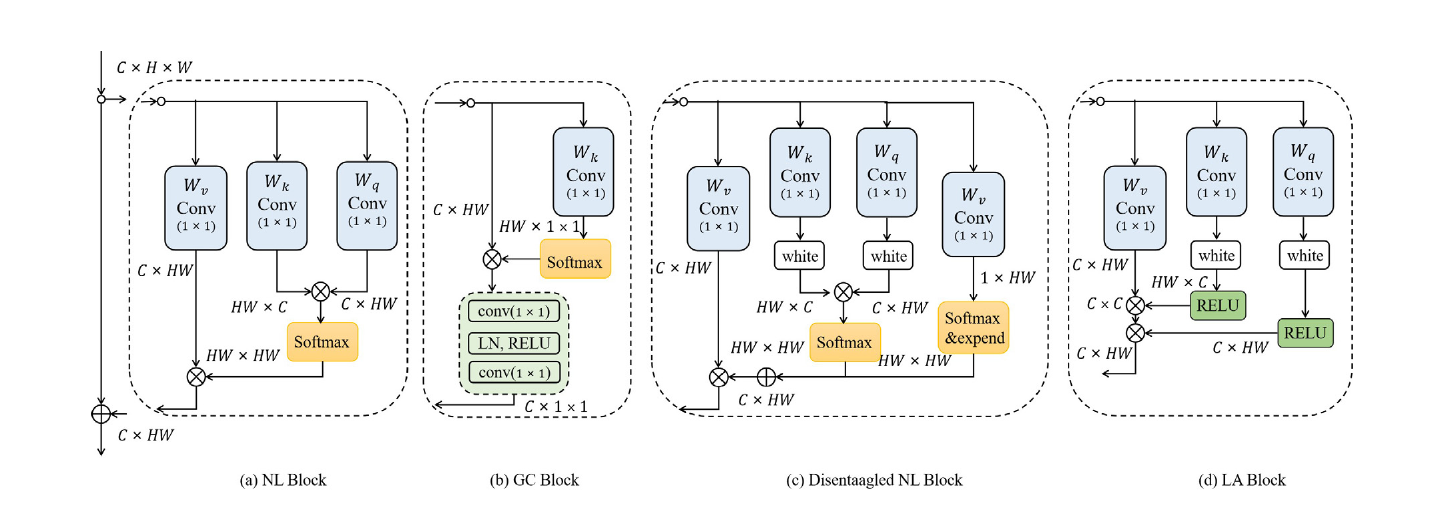
\includegraphics[width=0.9\linewidth]{img/LSNET_ATTN.png}
			\caption{Блоки внимания NL, GC, Disentangled NL и линейный блок LA в LSNet \cite{lsnet}}
			\label{lsnetattn}
		\end{figure}

		В RTLinearFormer \cite{rtlinearformer} ядро тоже ReLU, но к нему добавлены блоки на матрицах запросов ключей и
		значений и многомасштабные токены через глубинную свертку, а на ветви высокого разрешения стоит перекрестное линейное внимание CRLA
		(см. рис. \ref{rtlfblock}).

		\begin{figure}[H]
			\center
			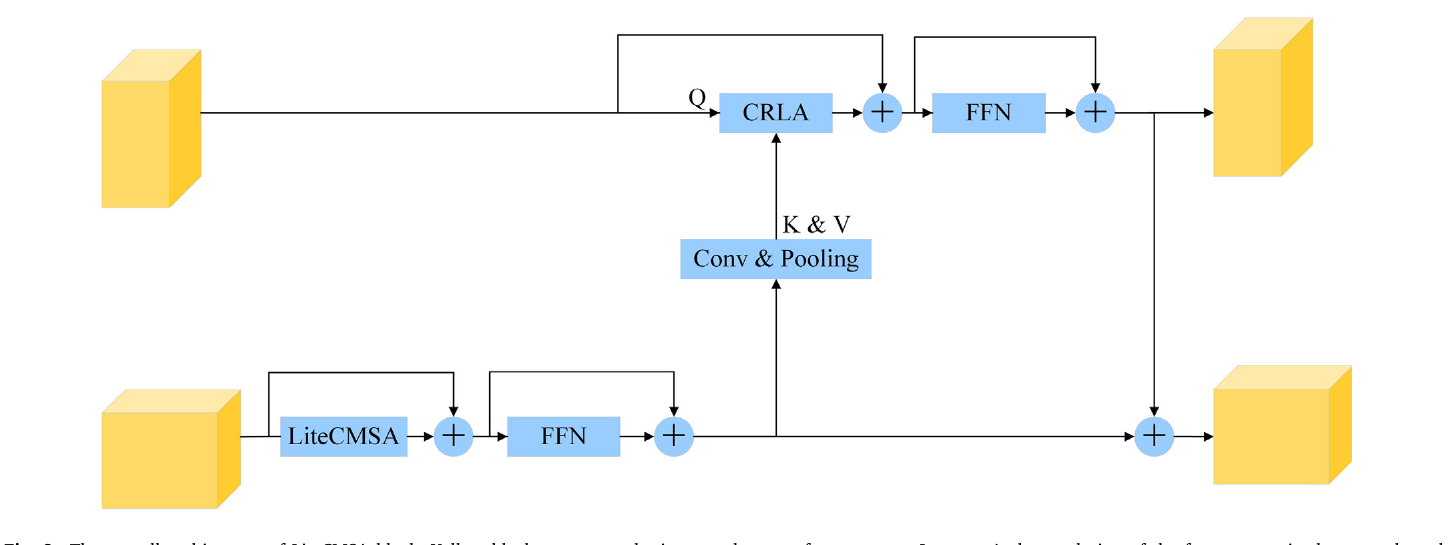
\includegraphics[width=0.8\linewidth]{img/RTLINEARFORMER_BLOCK.png}
			\caption{Блок LiteCMSA в RTLinearFormer \cite{rtlinearformer}}
			\label{rtlfblock}
		\end{figure}

		В GLANet \cite{glanet} ядро squareplus оно в отличии от ReLU не зануляет отрицательные значения и считается без
		экспонент, что должно ускорить механизм (см. рис. \ref{glanetarch}).

		\begin{figure}[H]
			\center
			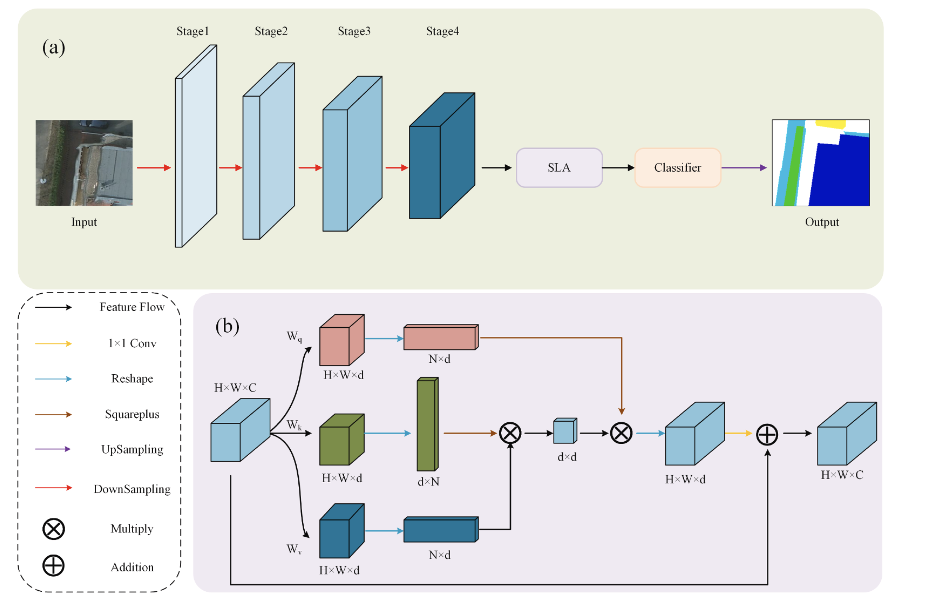
\includegraphics[width=0.7\linewidth]{img/GLANET_ARCH.png}
			\caption{Архитектура GLANet и модуль линейного внимания SLA \cite{glanet}}
			\label{glanetarch}
		\end{figure}

		В ABCFNet \cite{abcfnet} через softplus линеаризована только пространственная ветвь, а канальная оставлена
		на softmax, потому что каналов мало и квадратичность по ним не мешает (см. рис. \ref{abcfdca}).

		\begin{figure}[H]
			\center
			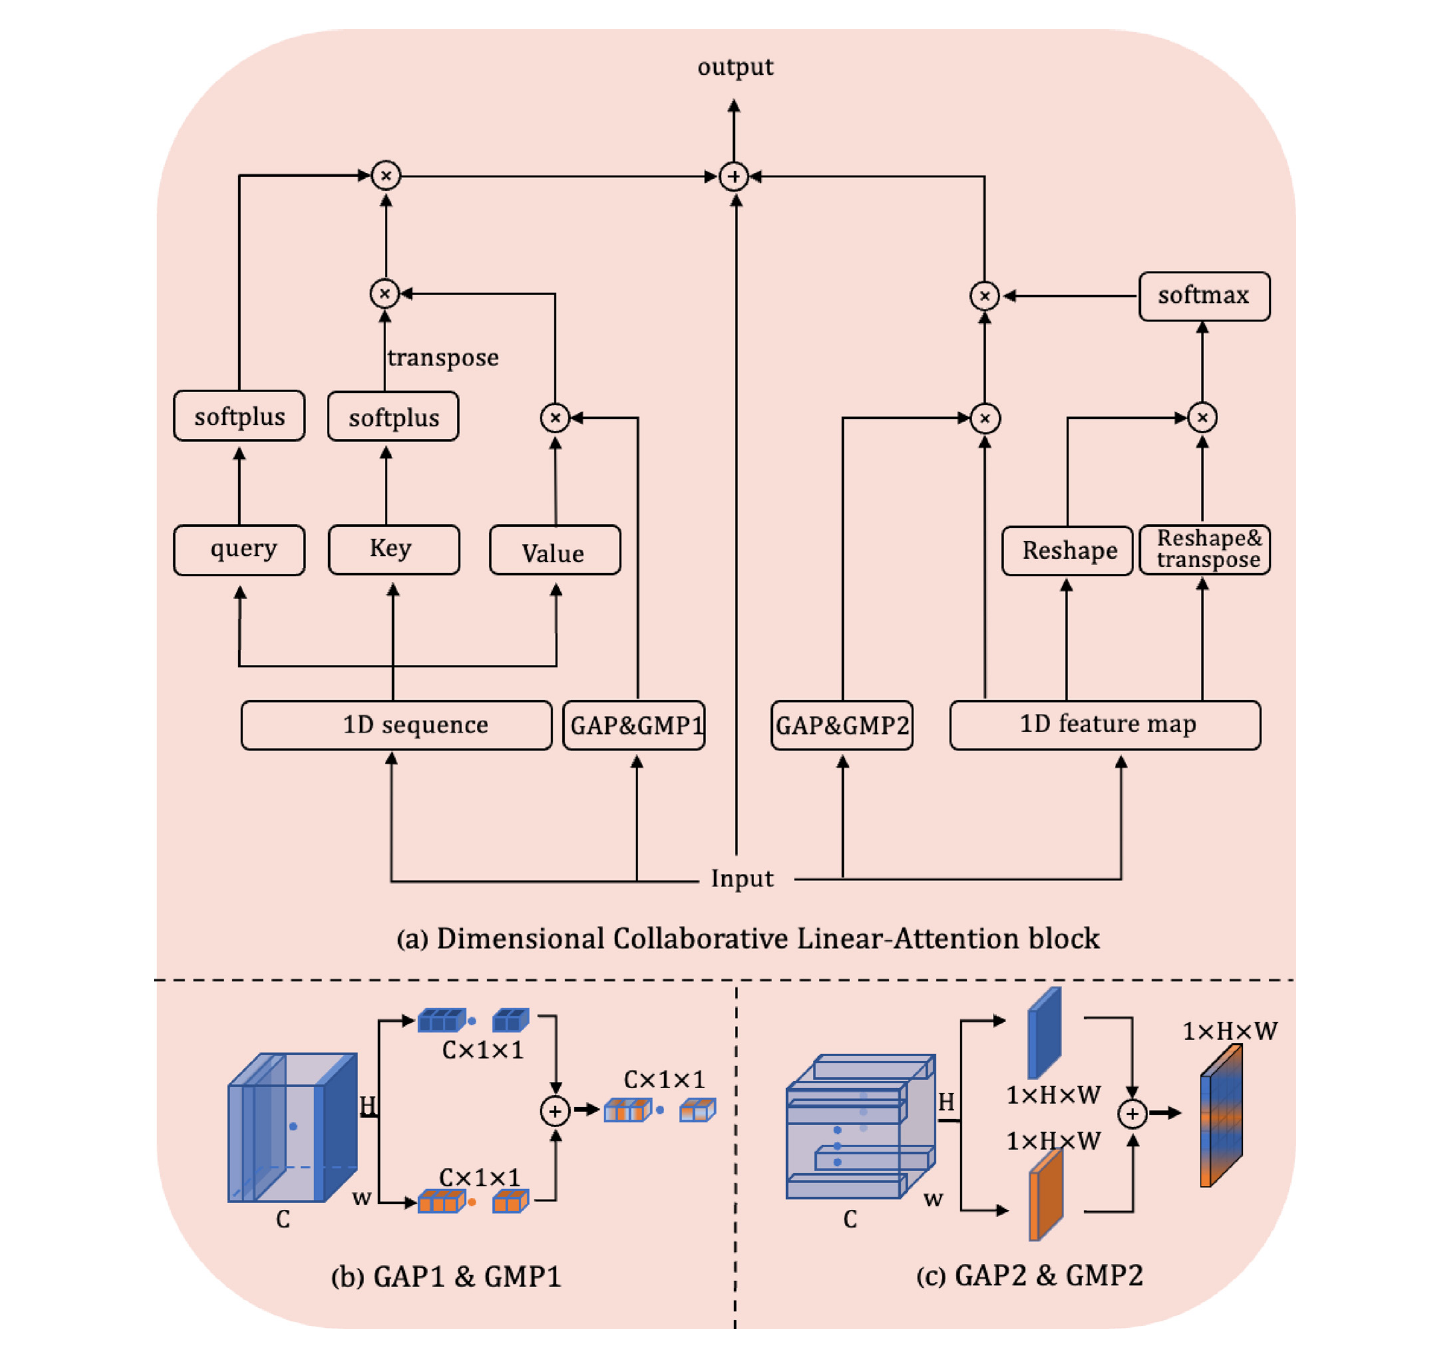
\includegraphics[width=0.6\linewidth]{img/ABCFNET_DCA.png}
			\caption{Модуль DCA в ABCFNet, слева линейная пространственная ветвь справа канальная \cite{abcfnet}}
			\label{abcfdca}
		\end{figure}

		В MLFormer \cite{mlformer} и WTP-MILA-UNet
		\cite{wtpmilaunet} используется Mamba-подобное внимание MLLA с ядром ELU и гейтом на SiLU (см. рис. \ref{mlformerarch}), причем сканирования
		последовательности тут нет и все токены считаются параллельно.

		\begin{figure}[H]
			\center
			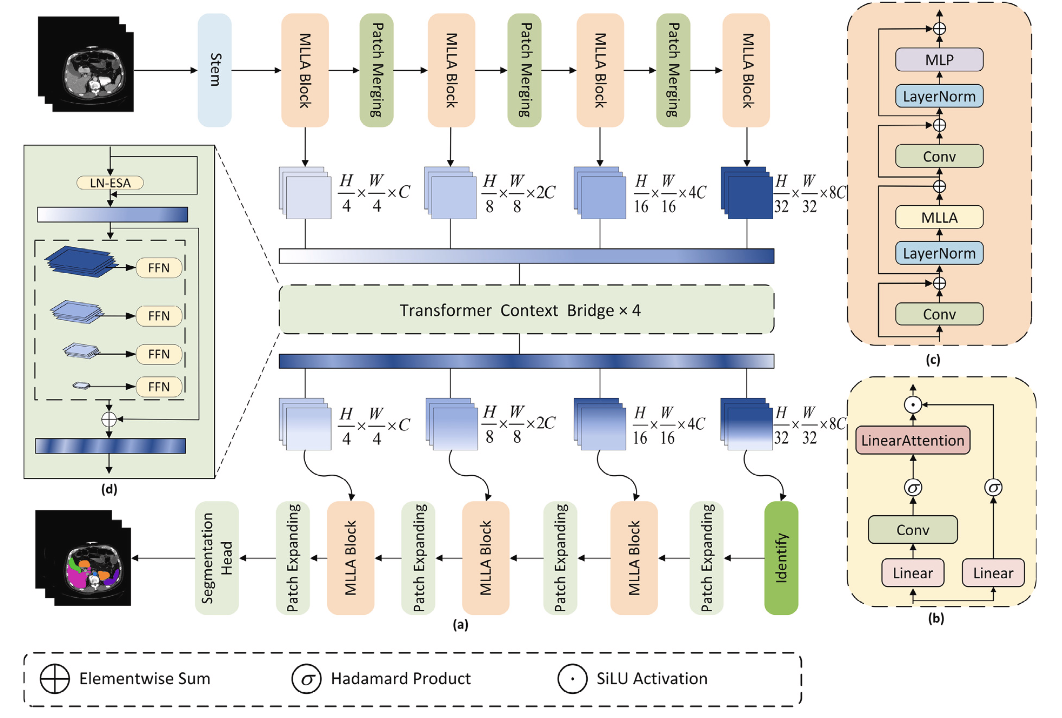
\includegraphics[width=0.8\linewidth]{img/MLFORMER_ARCH.png}
			\caption{Архитектура MLFormer и блок MLLA \cite{mlformer}}
			\label{mlformerarch}
		\end{figure}

		В MS-LCFNet \cite{mslcfnet} ядро кубическое - оно притягивает векторы к осям и делает
		распределение весов точнее. В UUEKAN \cite{uuekan} взято внимание MALA с компенсацией нормы, которое возвращает информацию о величине сходства
		теряемую без softmax.





		Третье это другие приближения softmax внимания, без замены его ядром. В CLT-MambaSeg \cite{cltmambaseg} ключи и значения проецируются
		в $k$ токенов как в Linformer и сложность становится $O(Nk)$ (см. рис. \ref{cltarch}).

		\begin{figure}[H]
			\center
			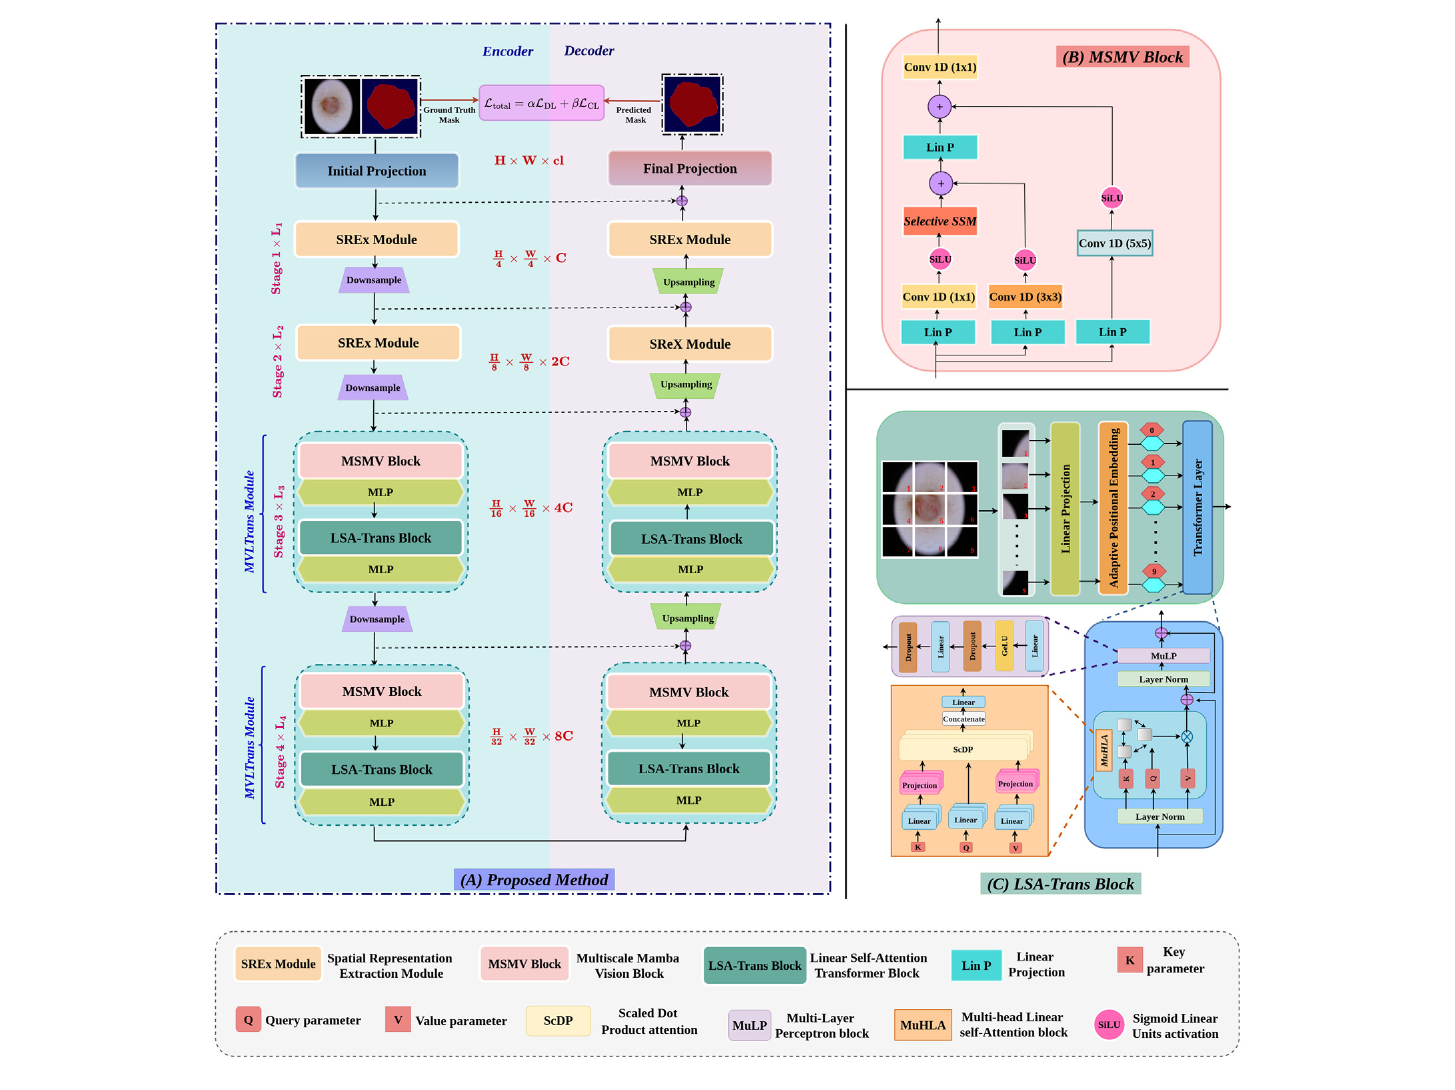
\includegraphics[width=0.85\linewidth]{img/CLTMAMBA_ARCH.png}
			\caption{Архитектура CLT-MambaSeg, блок MSMV и блок LSA-Trans с линейным вниманием \cite{cltmambaseg}}
			\label{cltarch}
		\end{figure}

		В PMP \cite{pmp} попарные сходства не считаются вообще.
		Обучаемый вектор весов сворачивает запросы в один глобальный вектор который потом поэлементно модулирует ключи (см. рис. \ref{pmpattn}). 
		Транспонированное внимание строит матрицу между каналами и теряет
		пространственную локализацию а разделимое внимание накладывает на пространственную карту ограничение.

		\begin{figure}[H]
			\center
			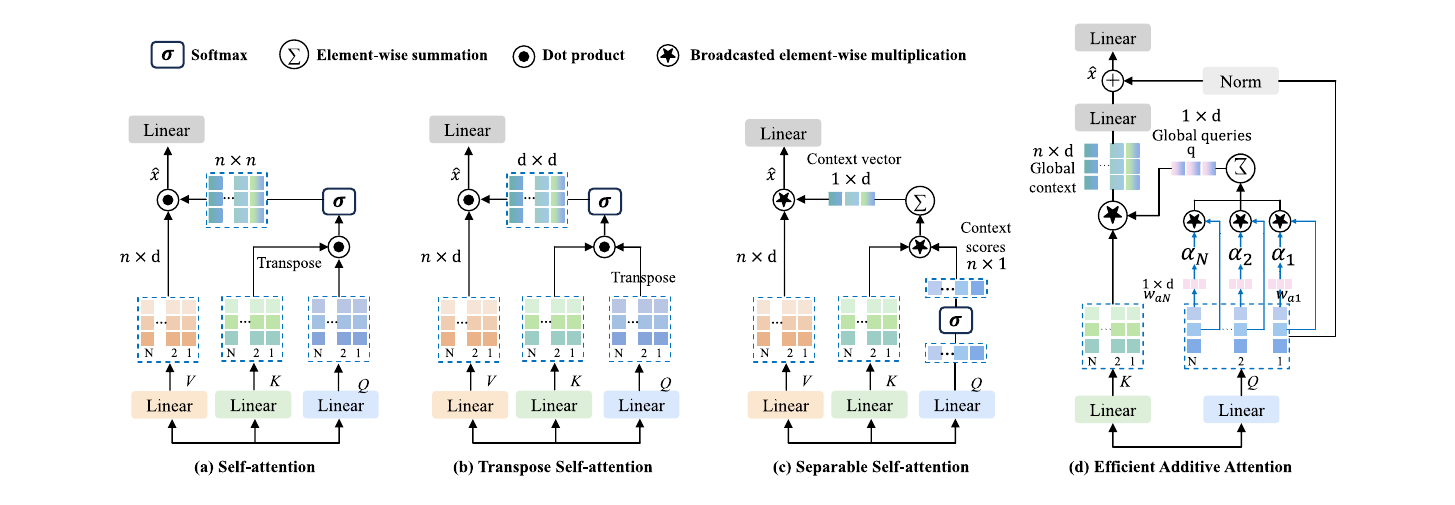
\includegraphics[width=0.95\linewidth]{img/PMP_ATTN.png}
			\caption{Механизмы внимания в работе PMP, (a) самовнимание (b) транспонированное (c) разделимое (d) аддитивное \cite{pmp}}
			\label{pmpattn}
		\end{figure}

		В HLSM-ViT \cite{hlsmvit} softmax оставлен но считается только на $m$ важных токенах,
		 при $m$ порядка $2\sqrt{N}$ это дает линейную сложность, и такая ветвь работает
		вместе с фокусированным линейным вниманием и глубинной сверткой (см. рис. \ref{hlsmarch}).

		\begin{figure}[H]
			\center
			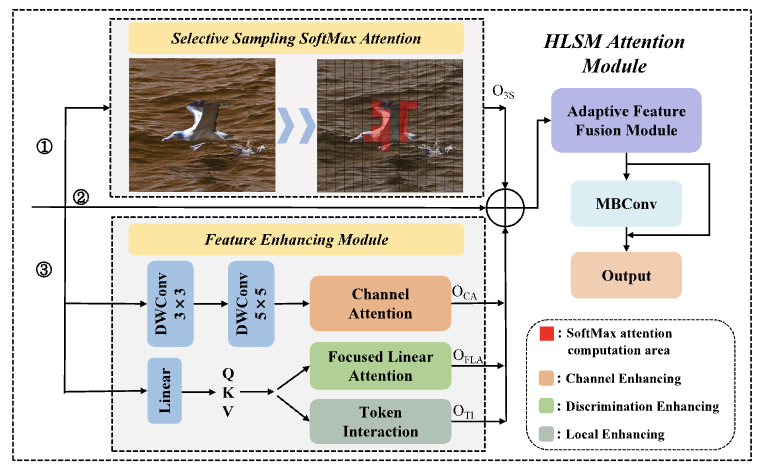
\includegraphics[width=0.7\linewidth]{img/HLSM_ARCH.png}
			\caption{Модуль гибридного внимания HLSM \cite{hlsmvit}}
			\label{hlsmarch}
		\end{figure}

		Четвертое семейство это модели пространства состояний и RWKV со сканированием последовательности. Тут линейность в отличии от предыдущих 
		статей получается не из формы внимания а из рекуррентного прохода по токенам. 
		MASA-VMUNet \cite{masavmunet} использует VMamba с четырьмя направлениями сканирования, CLT-MambaSeg
		\cite{cltmambaseg} ставит блоки MambaVision перед линейным трансформером. В статье про сеть Snake-RWKV \cite{snakerwkv} берет двунаправленный оператор.
		Snake-RWKV \cite{snakerwkv} отличается тем что направления сканирования у него непрерывные, то есть путь идет змейкой и соседние пиксели остаются
		соседями в последовательности (см. рис. \ref{snakescan}), а сдвиг токенов обучается подстраиваться под изгиб сосуда.

		\begin{figure}[H]
			\center
			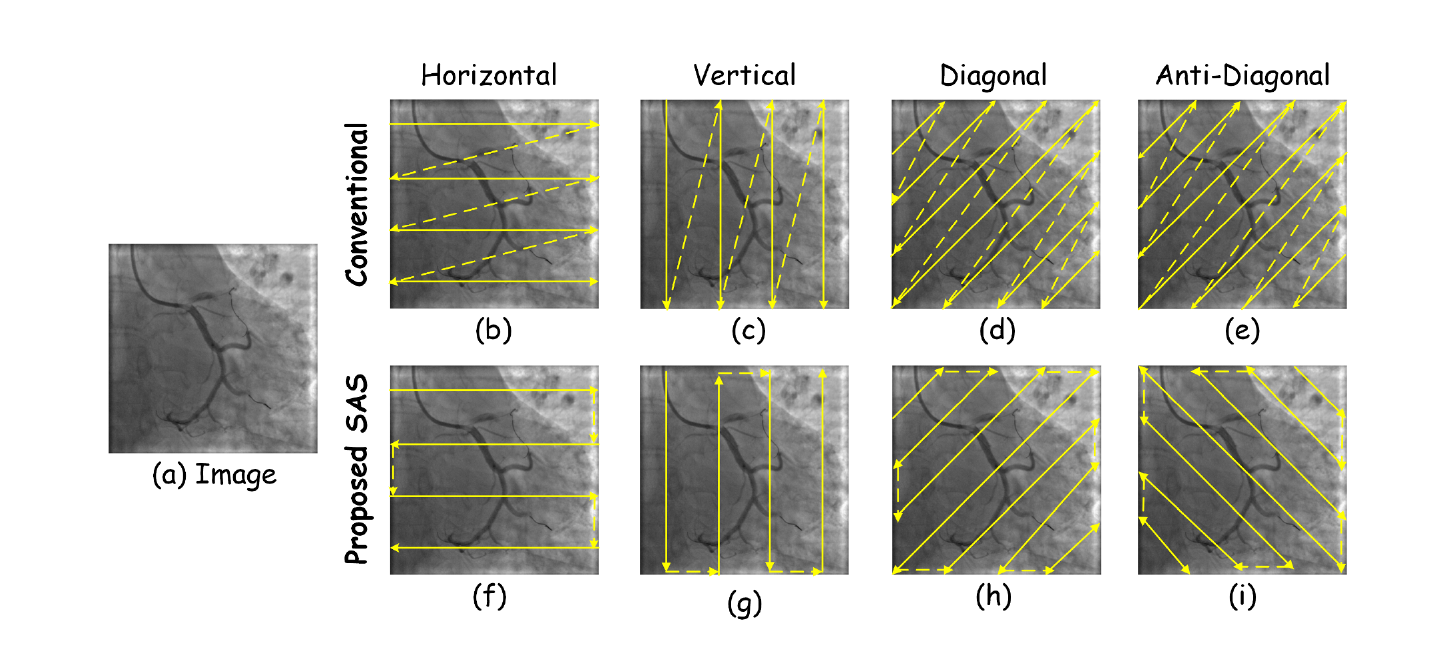
\includegraphics[width=0.9\linewidth]{img/SNAKERWKV_SCAN.png}
			\caption{Обычное сканирование сверху и непрерывное сканирование SAS в Snake-RWKV снизу \cite{snakerwkv}}
			\label{snakescan}
		\end{figure}

		Пятое отдельно, потому что эти механизмы называются линейными но линейности по числу пикселей у них нет. В LPT-Net
		\cite{lptnet} обычное softmax внимание считается внутри каждой строки карты признаков, а между строками информация передается небольшими окнами
		(см. рис. \ref{lptblock}). Сложность такого блока квадратична по ширине изображения, то есть это скорее полосовое внимание.

		\begin{figure}[H]
			\center
			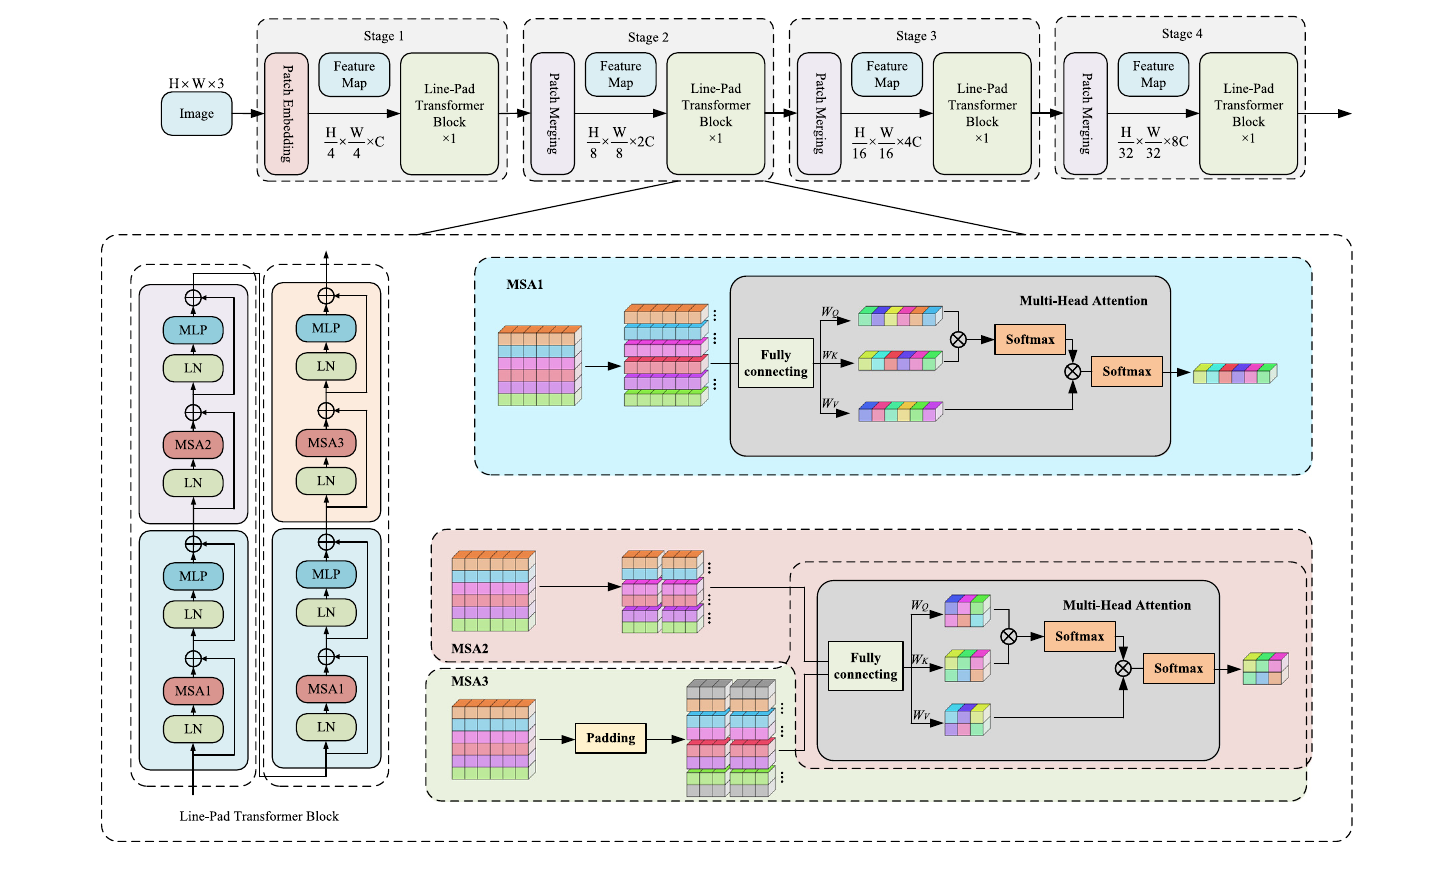
\includegraphics[width=0.9\linewidth]{img/LPTNET_BLOCK.png}
			\caption{Архитектура LPT-Net и блок Line-Pad Transformer \cite{lptnet}}
			\label{lptblock}
		\end{figure}

		В CA-UNet
		\cite{caunet} матрица внимания строится между каналами (см. рис. \ref{caunetmasa}), сложность по пикселям тут линейна но
		пиксели напрямую друг с другом не взаимодействуют и глобальный контекст идет только через статистики каналов. Именно этот вариант в PMP
		\cite{pmp} и отвергли из-за потери локализации.

		\begin{figure}[H]
			\center
			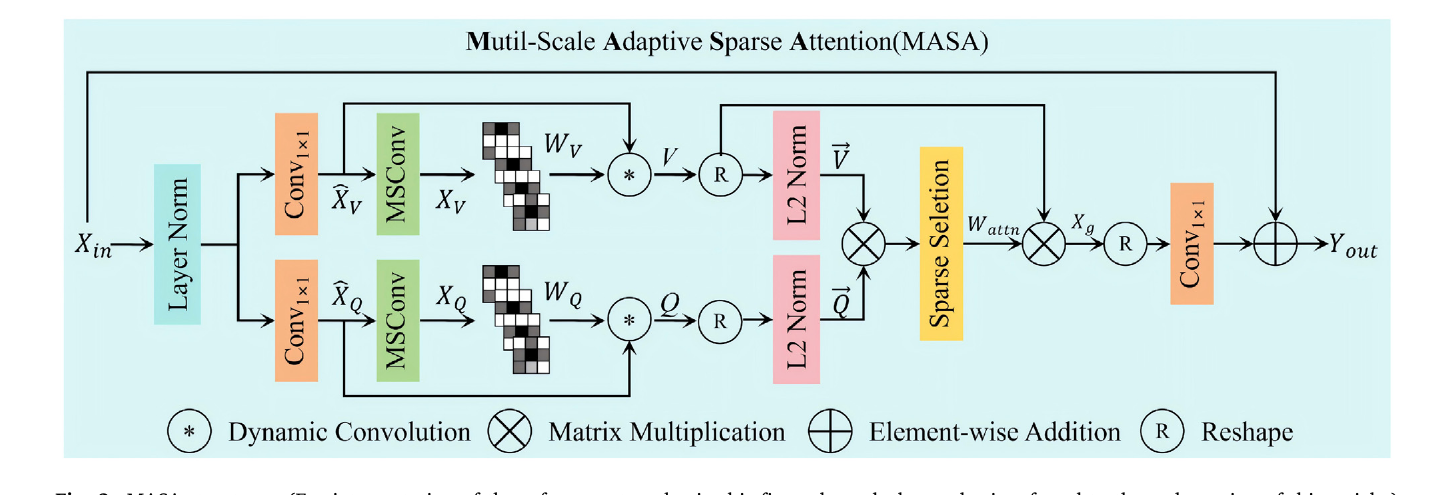
\includegraphics[width=0.85\linewidth]{img/CAUNET_MASA.png}
			\caption{Модуль канального внимания MASA в CA-UNet \cite{caunet}}
			\label{caunetmasa}
		\end{figure}

		Для переноса в SegFormer подходит только ядерное линейное внимание, так как два других варианта
		меняют сами связи между пикселями.


	\subsection{Линейное внимание в архитектуре}
		В подглаве рассуждается куда именно ставится линейный механизм так как тут тоже в разных статьях разные рекомендации. В SegFormer внимание стоит во всех
		блоках кодировщика. В LSNet блок линейного внимания ставится после первой и четвертой стадии ResNet-18, в RTLinearFormer
		 трансформерные блоки занимают только две последние стадии а первые остаются сверточными, в HLSM-ViT модуль
		работает на третьей и четвертой стадии. В GLANet линейное внимание вообще одно на всю сеть и стоит после сверточного кодировщика.
		ABCFNet наоборот ставит модуль после каждой из четырех стадий, то есть линейное внимание работает и на высоком разрешении.
		В медицинских работах тоже самое - в статье про MLFormer блоки MLLA образуют весь кодировщик и декодировщик, в CLT-MambaSeg
		 линейный трансформер стоит на третьей и четвертой стадии, в Snake-RWKV на двух последних стадиях и в
		декодировщике, а в UUEKAN только на skip соединениях в ResNet.

		То есть - линейное внимание ставят на глубоких стадиях с низким разрешением где оно дает глобальный контекст, а
		детали на высоком разрешении оставляют сверткам. В GLANet это проверили отдельно, модуль на последней стадии дает 74.80\% mIoU, а на
		всех стадиях сразу 74.75\% при большем числе параметров и большем времени обучения.

		Второе общее решение это то что чистое линейное внимание почти никогда не используется само по себе. Его дополняют сверточными ветвями и гейтами
		\cite{mlformer, rtlinearformer, abcfnet}, небольшим числом softmax токенов \cite{hlsmvit}, фокусирующим или компенсирующим ядром
		\cite{mslcfnet, uuekan}, а также перекрестным вниманием в декодировщике \cite{lsnet, pmp}. Это косвенно подтверждает что после линеаризации сети
		чего-то не хватает, и дальше это видно уже по результатам.

	\subsection{Точность линейного и квадратичного внимания}
		Главне в статьях те эксперименты где линейное внимание сравнивается с квадратичным внутри одной и той же
		архитектуры. Таких проверок всего несколько и причем результаты разные. Так же сама линеаризация может 
		просто потерять точность.

		В GLANet линейный модуль SLA сравнивается и с обычным скалярным вниманием и с другими линейными приближениями. 
		По вычислениям еть разница - на входе $128 \times 128$ скалярное внимание требует 2.1 GFLOPs и 16.5 Гб памяти а SLA всего 84 млн FLOPs и 44 Мб
		(см. таб. \ref{tab:glanet2}). При этом по точности SLA обходит Linformer, Luna и Efficient Attention на обоих датасетах ISPRS
		(см. таб. \ref{tab:glanet3}) а прирост относительно базовой модели составляет 0.56\% mIoU на Potsdam и 1.38\% на Vaihingen.

		% a global linear 7, (2, 3)
		\begin{table}[H]
			\centering
			\footnotesize
			\caption{Вычислительная стоимость скалярного внимания DPA и линейного внимания SLA при разных размерах входа \cite{glanet}}
			\label{tab:glanet2}
			\begin{tabular}{llcc}
				\toprule
				Method & Input length & FLOPs & Memory \\
				\midrule
				\multirow{3}{*}{DPA} & $32 \times 32$ & 134M & 86M \\
				 & $64 \times 64$ & 537M & 1.1G \\
				 & $128 \times 128$ & 2.1G & 16.5G \\
				\midrule
				\multirow{3}{*}{SLA} & $32 \times 32$ & 5M & 2M \\
				 & $64 \times 64$ & 21M & 8M \\
				 & $128 \times 128$ & 84M & 44M \\
				\bottomrule
			\end{tabular}
		\end{table}

		\begin{table}[H]
			\centering
			\footnotesize
			\caption{Сравнение SLA с другими методами линейного внимания на датасетах ISPRS \cite{glanet}}
			\label{tab:glanet3}
			\begin{tabular}{llccc}
				\toprule
				Dataset & Method & mF1(\%) & OA(\%) & mIoU(\%) \\
				\midrule
				\multirow{5}{*}{Potsdam} & backbone & 84.56 & 87.68 & 74.24 \\
				 & +Linformer & 84.65 & 87.83 & 74.46 \\
				 & +Luna & 84.55 & 87.74 & 74.22 \\
				 & +Efficient Attention & \underline{84.72} & \underline{87.95} & \underline{74.62} \\
				 & +SLA & \textbf{84.94} & \textbf{88.10} & \textbf{74.80} \\
				\midrule
				\multirow{5}{*}{Vaihingen} & backbone & 80.47 & 84.59 & 68.31 \\
				 & +Linformer & 80.69 & 84.71 & 68.46 \\
				 & +Luna & \underline{81.53} & 85.20 & \underline{69.42} \\
				 & +Efficient Attention & 81.25 & \underline{85.33} & 69.41 \\
				 & +SLA & \textbf{81.70} & \textbf{85.43} & \textbf{69.69} \\
				\bottomrule
			\end{tabular}
		\end{table}

		В ABCFNet \cite{abcfnet} такое же сравнение сделано уже с замером скорости  (см. таб. \ref{tab:abcfattn}). Модуль DCA
		работает с той же скоростью что и простое ядерное линейное внимание и точнее его на 1.34\% MIoU. Полное внимание трансформера втрое медленнее при
		22.2 кадра в секунду и при этом не точнее. Однако оконное внимание Swin дает на 0.6\% больше MIoU чем DCA хотя и работает медленнее. То есть
		линейное внимание выигрывает в балансе но не в чистой точности.

		% shallow 16, 7
		\begin{table}[H]
			\centering
			\footnotesize
			\caption{Сравнение механизмов внимания при одинаковом кодировщике на датасете Potsdam \cite{abcfnet}}
			\label{tab:abcfattn}
			\setlength{\tabcolsep}{4pt}
			\begin{adjustbox}{max width=\linewidth}
			\begin{tabular}{lcccccc}
				\toprule
				\multirow{2}{*}{Model} & \multicolumn{3}{c}{Potsdam} & \multirow{2}{*}{Params (M)} & \multirow{2}{*}{FLOPs (G)} & \multirow{2}{*}{FPS $\uparrow$} \\
				\cmidrule(lr){2-4}
				 & MIoU (\%) & mPA (\%) & Acc (\%) & & & \\
				\midrule
				Baseline & 83.94 & 90.86 & 94.23 & 28.89 & 28.3146 & 82.83 \\
				+CBAM & 84.26 & 92.20 & 94.39 & $31.02_{(+2.13)}$ & $28.3181_{(+0.00)}$ & 82.79 \\
				+SE & 84.12 & 92.17 & 93.98 & $29.58_{(+0.69)}$ & $28.3215_{(+0.01)}$ & 82.80 \\
				+kernel attention & 86.14 & 93.57 & 94.92 & $35.86_{(+6.97)}$ & $33.6923_{(+5.38)}$ & 64.43 \\
				+LinformerBlock & 85.96 & 93.31 & 94.83 & $38.34_{(+9.45)}$ & $38.6712_{(+10.36)}$ & 55.62 \\
				+Swin-attention & 88.09 & 94.31 & 95.83 & $46.30_{(+17.41)}$ & $46.8926_{(+18.58)}$ & 43.81 \\
				+Transformer & 87.22 & 94.13 & 95.32 & $51.91_{(+23.02)}$ & $124.0251_{(+95.71)}$ & 22.17 \\
				+DCA & 87.48 & 94.09 & 95.67 & $35.86_{(+6.97)}$ & $33.7002_{(+5.39)}$ & 64.42 \\
				\bottomrule
			\end{tabular}
			\end{adjustbox}
		\end{table}

		В медицинских работах линеаризация обходится вычислительно дешевле. В CLT-MambaSeg замена самовнимания на линейное почти не меняет качество
		и снижает FLOPs с 8.55 до 7.02 G (см. таб. \ref{tab:clt8}). В MLFormer замена многоголового внимания на MLLA даже повышает Dice с
		77.91\% до 79.24\% и снижает FLOPs более чем вдвое (см. таб. \ref{tab:mlformerabl}). В PMP сравнивали целые кодировщики и там
		аддитивное внимание обошло ViT кодировщик с квадратичным вниманием - 89.69\% против 88.33\% mIoU при одинаковом базовом декодировщике. Похоже что
		на небольших входах вроде $224 \times 224$ и при малом числе классов линейное внимание вообще ничего не теряет.

		% clt mambaseg 20, 8
		\begin{table}[H]
			\centering
			\footnotesize
			\caption{Влияние типа внимания в блоке LSA-Trans на качество сегментации \cite{cltmambaseg}}
			\label{tab:clt8}
			\begin{tabular}{lcccccc}
				\toprule
				\multirow{2}{*}{Attention type} & \multicolumn{3}{c}{ISIC-2016} & \multicolumn{3}{c}{BUSI} \\
				\cmidrule(lr){2-4} \cmidrule(lr){5-7}
				 & IoU & DS & FLOPs (G) & IoU & DS & FLOPs (G) \\
				\midrule
				Self-Attention & 90.98 & 92.91 & 8.55 & 92.20 & 92.29 & 8.55 \\
				Linear-Attention & 91.05 & 92.96 & 7.02 & 92.19 & 92.32 & 7.02 \\
				\bottomrule
			\end{tabular}
		\end{table}

		% mlformer 14, 7
		\begin{table}[H]
			\centering
			\footnotesize
			\caption{Абляция модулей Stem, MLLA и моста на датасете Synapse \cite{mlformer}}
			\label{tab:mlformerabl}
			\setlength{\tabcolsep}{4pt}
			\begin{adjustbox}{max width=\linewidth}
			\begin{tabular}{ccccccccc}
				\toprule
				\multicolumn{4}{l}{Modules} & \multicolumn{5}{l}{Performance/Complexity} \\
				\cmidrule(r){1-4} \cmidrule(l){5-9}
				Base & Stem & MLLA & Transformer bridge & DSC (\%)$\uparrow$ & HD95 (mm)$\downarrow$ & Params (M) & FLOPs (G) & IT (ms) \\
				\midrule
				$\checkmark$ & & & & 77.91 & 28.29 & 19.31 & 8.54 & 10.32 \\
				 & $\checkmark$ & & & 78.33 & 22.92 & 19.49 & 10.52 & 10.48 \\
				 & & $\checkmark$ & & 79.24 & 24.41 & 17.61 & 3.82 & 11.95 \\
				 & & & $\checkmark$ & 80.41 & 21.20 & 34.46 & 13.25 & 15.05 \\
				 & $\checkmark$ & $\checkmark$ & & 80.60 & 24.96 & 17.78 & 4.52 & 12.05 \\
				 & $\checkmark$ & & $\checkmark$ & 81.05 & 27.95 & 34.57 & 13.77 & 15.06 \\
				 & & $\checkmark$ & $\checkmark$ & 82.38 & 21.09 & 32.76 & 8.53 & 15.62 \\
				 & $\checkmark$ & $\checkmark$ & $\checkmark$ & \textbf{83.07} & \textbf{15.77} & 32.86 & 9.04 & 15.63 \\
				\bottomrule
			\end{tabular}
			\end{adjustbox}
		\end{table}

		В сегментации сцен все наоборот. В RTLinearFormer замена линейного перекрестного внимания на обычное поднимает mIoU на
		0.45\% и теряет скорость с 66.7 до 56.4 кадра в секунду (см. таб. \ref{tab:rtlfattn}). В HLSM-ViT та же сеть с чистым линейным
		вниманием проигрывает гибридной около одного пункта $AP^m$ на экземплярной сегментации COCO (см. таб. \ref{tab:hlsm6}), причем заметнее всего
		разрыв на мелких объектах, при этом авторы статьи говорят что это из-за того что средний ранг карты внимания у гибридного механизма полный, а у линейного только 71.
		Получается что цена линеаризации зависит от задачи.

		% rtlinearform 9, 9
		\begin{table}[H]
			\centering
			\footnotesize
			\caption{Сочетания механизмов внимания в RTLinearFormer на Cityscapes \cite{rtlinearformer}}
			\label{tab:rtlfattn}
			\begin{tabular}{lcc}
				\toprule
				Attention combination & FPS & mIoU(\%) \\
				\midrule
				LMSA+CRLA & 65.5 & 78.30 \\
				LiteCMSA+CA & 56.4 & 78.86 \\
				LiteCMSA+CRLA & 66.7 & 78.41 \\
				\bottomrule
			\end{tabular}
		\end{table}

		% hybrid linear attention 9, 6
		\begin{table}[H]
			\centering
			\footnotesize
			\caption{Экземплярная сегментация на COCO 2017, гибридное внимание против чистого линейного \cite{hlsmvit}}
			\label{tab:hlsm6}
			\setlength{\tabcolsep}{4pt}
			\begin{tabular}{lcccccccc}
				\toprule
				\multicolumn{9}{l}{Mask R-CNN instance segmentation on COCO} \\
				\midrule
				 & Param & Schedule & $AP^m$ & $AP^m_{50}$ & $AP^m_{75}$ & $AP^m_s$ & $AP^m_m$ & $AP^m_l$ \\
				\midrule
				S3ML-ViT-M1 & 4.4 & 1x & \underline{31.3} & \underline{51.5} & \underline{33.1} & 14.5 & 33.1 & \underline{45.9} \\
				HLSM-ViT-M1-Linear & 4.0 & 1x & 31.2 & 51.1 & \underline{33.1} & \underline{14.7} & \underline{33.5} & 45.6 \\
				\textbf{HLSM-ViT-M1(ours)} & 4.3 & 1x & \textbf{32.3} & \textbf{53.0} & \textbf{34.2} & \textbf{14.8} & \textbf{34.5} & \textbf{47.3} \\
				\midrule
				PVT-T & 13.2 & 1x & 35.1 & 56.7 & 37.3 & \textbf{19.5} & 37.4 & 48.5 \\
				S3ML-ViT-M3 & 9.0 & 1x & 35.1 & 56.4 & 37.4 & 17.0 & \underline{37.8} & 50.8 \\
				HLSM-ViT-M3-Linear & 7.8 & 1x & \underline{35.4} & \underline{57.0} & \underline{37.8} & 17.9 & 37.7 & \underline{51.1} \\
				\textbf{HLSM-ViT-M3(ours)} & 8.6 & 1x & \textbf{36.6} & \textbf{58.5} & \textbf{38.7} & \underline{18.1} & \textbf{39.4} & \textbf{52.4} \\
				\bottomrule
			\end{tabular}
		\end{table}

	\subsection{Скорость инференса и задержка}
		По скорости работы делятся на две части. В сегментации сцен линеаризация действительно делает трансформер работающий в реальном времени.
		LSNet \cite{lsnet} дает 73.94\% mIoU при 130.2 кадра в секунду на Cityscapes, RTLinearFormer \cite{rtlinearformer} 78.41\% при 66.7 кадра на
		полном разрешении $1024 \times 2048$, тогда как SegFormer-B0 \cite{segformer} на близкой задаче работает с 15.2 кадра при короткой стороне 1024
		пикселя. Прямое сопоставление есть в RTLinearFormer на ADE20K, где обе модели меряли на одной RTX 3090. Переход от
		внимания с понижением размерности к линейному дал ускорение в 1.3 раза ценой 1.7\% mIoU. Сводка по этим работам собрана в
		таблице \ref{tab:rtcompare}, там же указаны условия замера, так как видеокарты и разрешения у авторов разные.

		% segformer (1, 2), lsnet (2, 3), rtlinearformer (2, 3, 4)
		\begin{table}[H]
			\centering
			\footnotesize
			\caption{Сводное сравнение сегментаторов реального времени по данным статей \cite{segformer, lsnet, rtlinearformer}}
			\label{tab:rtcompare}
			\begin{adjustbox}{max width=\linewidth}
			\begin{tabular}{llcccccc}
				\toprule
				Модель & Внимание & Датасет & Разрешение & mIoU (\%) & FPS & GPU & GFLOPs \\
				\midrule
				SegFormer-B0 & ESA, $O(N^2/R)$ & Cityscapes val & короткая сторона 1024 & 76.2 & 15.2 & V100 & 125.5 \\
				SegFormer-B0 & ESA, $O(N^2/R)$ & Cityscapes val & короткая сторона 512 & 71.9 & 47.6 & V100 & 17.7 \\
				LSNet & ReLU, $O(N)$ & Cityscapes test & $1024 \times 1024$ & 73.94 & 130.2 & RTX 3080 & - \\
				RTLinearFormer & ReLU, $O(N)$ & Cityscapes val & $1024 \times 2048$ & 78.41 & 66.7 & RTX 3090 & 117.68 \\
				DDRNet-23 & нет & Cityscapes val & $1024 \times 2048$ & 79.5 & 51.4 & RTX 3090 & 143.1 \\
				RTFormer-Base & внешнее, $O(N)$ & Cityscapes val & $1024 \times 2048$ & 79.3 & 56.1 & RTX 3090 & 145.0 \\
				\midrule
				LSNet & ReLU, $O(N)$ & CamVid test & $720 \times 960$ & 72.3 & 104.53 & RTX 3080 & - \\
				RTLinearFormer & ReLU, $O(N)$ & CamVid test & $720 \times 960$ & 77.4 & 143.2 & RTX 3090 & - \\
				\midrule
				SegFormer-B0 & ESA, $O(N^2/R)$ & ADE20K val & $512 \times 512$ & 37.4 & 84.4 & RTX 3090 & - \\
				RTLinearFormer & ReLU, $O(N)$ & ADE20K val & $512 \times 512$ & 35.7 & 107.3 & RTX 3090 & 14.74 \\
				\bottomrule
			\end{tabular}
			\end{adjustbox}
		\end{table}

		Во второй части работ измеряют по другому так как снижение FLOPs не всегда переходит в снижение задержки. В MLFormer
		\cite{mlformer} линейное внимание вдвое дешевле по FLOPs чем обычное но время инференса при этом растет с 10.32 до 11.95 мс. В Snake-RWKV
		\cite{snakerwkv} задержка модели 34.23 мс, тогда как TransUNet с квадратичным вниманием и втрое большими FLOPs укладывается в 15.74 мс а обычный
		UNet в 9.26 мс (см. таб. \ref{tab:snake11}). Сами авторы объясняют это перестановками индексов и обратными отображениями при многонаправленном
		сканировании. В UUEKAN \cite{uuekan} модель при 9.35 GFLOPs работает всего с 9.5 кадра в секунду. В CA-UNet \cite{caunet} реальным временем
		называют 0.17 с на изображение, то есть около 6 кадров, а в MS-LCFNet \cite{mslcfnet} получается 10.85 кадра при 46.82 млн параметров.
		Самая тяжелая тут FESS-SAM \cite{fesssam} с 4.1 кадра и 364.6 GFLOPs. То есть идея с использованием SAM-моделей тут отпадает. Так как по идее 
		еще добавлялся бы алгоритм который на протяжении всего видеопотока будет сегментировать объекты по входному запросу.

		% Topology 12 , 11.
		\begin{table}[H]
			\centering
			\footnotesize
			\caption{Параметры, FLOPs и реальная задержка на входе $512 \times 512$, средние Dice и IoU по четырем датасетам артерий \cite{snakerwkv}}
			\label{tab:snake11}
			\begin{tabular}{lcccccc}
				\toprule
				Method & Params(M)$\downarrow$ & FLOPs(G)$\downarrow$ & Latency(ms)$\downarrow$ & Mem.(MB)$\downarrow$ & Avg Dice(\%)$\uparrow$ & Avg IoU(\%)$\uparrow$ \\
				\midrule
				UNet & 17.26 & 160.44 & 9.26 & 597.72 & 78.01 & 64.18 \\
				Attention-UNet & 34.88 & 266.23 & 12.93 & 693.16 & 78.14 & 64.35 \\
				DeepLab V3+ & 59.33 & 88.28 & 7.98 & 297.74 & 75.82 & 61.40 \\
				CS2 Net & 8.92 & 49.99 & 3.66 & 336.32 & 75.05 & 60.31 \\
				TransUNet & 67.07 & 133.47 & 15.74 & 579.80 & 78.88 & 65.30 \\
				SwinUNet & 27.18 & 30.90 & 6.06 & 337.05 & 71.03 & 55.52 \\
				FRUNet & 7.37 & 235.60 & 17.29 & 865.27 & 74.33 & 59.49 \\
				De-dcgcn-ee & 14.38 & 401.52 & 28.46 & 1137.65 & 76.78 & 62.75 \\
				H2Former & 33.68 & 121.38 & 30.18 & 1736.98 & 76.73 & 62.70 \\
				EMCAD & 26.76 & 22.39 & 7.89 & 224.22 & 78.17 & 64.40 \\
				IMFF-net & 35.35 & 287.86 & 13.59 & 772.75 & 78.47 & 64.78 \\
				SCSegamba & 3.90 & 17.75 & 44.50 & 269.71 & 74.17 & 59.31 \\
				CCViM & 32.16 & 18.26 & 17.70 & 438.65 & 79.48 & 66.09 \\
				Snake-RWKV (Ours) & 12.61 & 45.21 & 34.23 & 366.40 & 80.85 & 68.04 \\
				\bottomrule
			\end{tabular}
		\end{table}

		Отсюда видно что выигрыш по времени дает не любая линейная сложность. Ядерное линейное внимание без сканирования действительно ускоряет сеть и
		только при большом числе токенов \cite{lsnet, rtlinearformer}, а модели со сканированием последовательности \cite{snakerwkv, masavmunet} и
		тяжелые дополнительные модули \cite{uuekan} проигрывают по задержке даже квадратичным сетям. Для магистерской работы будет учтено что решение о линеаризации
		нужно принимать по замеру задержки на целевом разрешении кадра.

	\subsection{Анализ результатов}
		Числа из разных статей почти не сравнимы между собой из-за нескольких вещей. Главная проблема тут что скорость измеряют на разных видеокартах от RTX 3060 в
		LPT-Net \cite{lptnet} до RTX 5090 в UUEKAN \cite{uuekan}, и на разных разрешениях. Даже одна и та же базовая модель у разных авторов получается
		разной. VM-UNet на Synapse дает 82.38\% DSC в таблице MLFormer \cite{mlformer} и 81.08\% в таблице MASA-VMUNet \cite{masavmunet}, поэтому разрыв
		около процента между самими предложенными моделями уже нельзя считать надежным (см. таб. \ref{tab:synapse}). На датасете BUSI разброс 
		от 74.23\% Dice в MLFormer \cite{mlformer} и 77.88\% в UUEKAN \cite{uuekan} до 92.32\% в CLT-MambaSeg \cite{cltmambaseg} что объясняется разными
		разбиениями, исключением нормальных снимков и генеративной аугментацией. Отдельно стоит отметить CA-UNet \cite{caunet}, где модель на 5 млн
		параметров без предобучения дает 50.26\% mIoU на ADE20K, то есть почти уровень SegFormer-B5 \cite{segformer} с 84.7 млн параметров. Такой
		результат вызывает немного сомнения...

		% mlformer 2, 3, masa-vnet 1, 3
		\begin{table}[H]
			\centering
			\footnotesize
			\caption{Результаты на Synapse и ACDC по данным двух статей \cite{mlformer, masavmunet}}
			\label{tab:synapse}
			\begin{tabular}{llcccc}
				\toprule
				Модель & Тип глобального механизма & DSC Synapse (\%) & DSC Synapse (\%) & DSC ACDC (\%) & GFLOPs \\
				 & & по MLFormer & по MASA-VMUNet & & \\
				\midrule
				TransUNet & самовнимание & 77.48 & 77.48 & 89.71 & 88.91 \\
				Swin-UNet & оконное внимание & 79.13 & 79.13 & 90.00 & 7.72 \\
				MISSFormer & эффективное внимание & 81.96 & 81.96 & 91.19 & 9.89 \\
				VM-UNet & VMamba & 82.38 & 81.08 & - & 4.11 \\
				MLFormer & MLLA & 83.07 & - & 91.37 & 9.04 \\
				MASA-VMUNet & VMamba и criss-cross & - & 84.36 & 92.29 & 4.53 \\
				\bottomrule
			\end{tabular}
		\end{table}

		По этой причине в обзоре полезны только те сравнения скорости которые сделаны внутри одной статьи по отдельности и при одинаковых остальных условиях.
		 Их собрано немного, зато они дают нормальные данные \cite{glanet, abcfnet, cltmambaseg, mlformer, rtlinearformer, hlsmvit, pmp}.

	\subsection{Тонкие протяженные объекты}
		Для задачи сегментации рельсов отдельный интерес представляют работы где объекты тонкие и длинные. Таких случаев четыре и они дают согласованный
		вывод.

		В ABCFNet \cite{abcfnet} это дороги на спутниковых снимках DeepGlobe. Модель получает 83.29\% IoU при 41.21 GFLOPs и обходит сверточных и
		трансформерных конкурентов (см. таб. \ref{tab:abcfnet3}), правда разрыв с UNet++ и CMTFNet всего 0.2-0.3\% IoU - то есть линейное внимание тут не
		дает преимущества. В LPT-Net \cite{lptnet} авторы прямо пишут что их сеть хуже работает именно на линейных предметах.
		В RTLinearFormer \cite{rtlinearformer} перечислены классы на которых сеть ошибается чаще всего и это столбы и растительность, а причиной авторы
		называют свой же механизм линейного внимания. В Snake-RWKV \cite{snakerwkv} ошибки остаются на тонких дистальных ветвях сосудов в местах
		бифуркаций и при низком контрасте.

		% Shallow 14,3
		\begin{table}[H]
			\centering
			\footnotesize
			\caption{Сегментация дорог на датасете DeepGlobe \cite{abcfnet}}
			\label{tab:abcfnet3}
			\begin{adjustbox}{max width=\linewidth}
			\begin{tabular}{lcccccc}
				\toprule
				Method & IoU (\%) & mPA (\%) & Acc (\%) & Params(M) & FLOPs(G) & Memory(G) \\
				\midrule
				UNet & 81.78 & 89.50 & 89.45 & 32.52 & 32.92 & 1.71 \\
				PSPNet & 81.63 & 89.27 & 89.19 & 36.26 & 37.88 & 1.77 \\
				DeepLabV3+ & 82.26 & 89.81 & 89.32 & 26.67 & 36.78 & 1.66 \\
				MANet & 82.43 & 90.77 & 90.90 & 35.86 & 33.69 & 2.27 \\
				UNet++ & 82.98 & 91.24 & 90.82 & 48.98 & 89.73 & 3.21 \\
				A2FPN & 82.82 & 90.15 & 89.58 & 26.71 & 41.06 & 2.19 \\
				CMTFNet & 83.13 & 90.94 & 91.73 & 50.07 & 47.91 & 2.36 \\
				MIFNet & 83.07 & \textbf{91.87} & 91.79 & 52.35 & 55.17 & 2.58 \\
				\midrule
				ABCFNet (ours) & \textbf{83.29} & 91.36 & \textbf{92.10} & \textbf{44.50} & \textbf{41.21} & 2.23 \\
				\bottomrule
			\end{tabular}
			\end{adjustbox}
		\end{table}

		Противоположный пример дает FESS-SAM \cite{fesssam}. Там кабели и контактный провод в тоннеле лучше всех выделяет тяжелая модель SAM с полным
		квадратичным вниманием и без всякого дообучения, среднее IoU по шести элементам 0.819 против 0.651 у SegFormer-B5 (см. таб. \ref{tab:fesssam11}).
		Но тут как говорилось ранее проблема в скорости работы - 4.1 кадра в секунду против 17.4 у SegFormer-B5 и 49.5 у UNet. 
		А еще узкие швы обделки тоннеля не выделяет даже SAM.
		Получается что на тонких объектах точность пока луше квадратичным вниманием.

		% FESS-SAM
		\begin{table}[H]
			\centering
			\footnotesize
			\caption{Вычислительная эффективность и среднее IoU по шести элементам тоннеля \cite{fesssam}}
			\label{tab:fesssam11}
			\begin{tabular}{lcccccc}
				\toprule
				Method & Params (M) & FLOPs (G) & Training time (h) & Inference Speed (ms) & FPS & Mean IoU \\
				\midrule
				UNet & 32 & 13.8 & 1.65 & 20.2 & 49.5 & 0.393 \\
				SegNext-L & 45.1 & 49.5 & 3.55 & 52.3 & 19.1 & 0.59 \\
				SegFormer-B5 & 84.6 & 99.7 & 3.54 & 57.5 & 17.4 & 0.651 \\
				ViT-Adapter & 35.5 & 227.9 & 1.98 & 59.8 & 16.7 & 0.765 \\
				YoLo-SAM & 138.8 & 372.2 & 2.27 & 145.4 & 6.9 & 0.701 \\
				FESS-SAM & 136 & 364.6 & N/A & 248 & 4.1 & 0.819 \\
				\bottomrule
			\end{tabular}
		\end{table}

		Snake-RWKV \cite{snakerwkv} при этом показывает что помогает не сама линеаризация а учет геометрии объекта. Замена обычного многонаправленного
		сканирования на непрерывное дает прибавку Dice от 0.23 до 0.44 пункта на четырех датасетах а обучаемый сдвиг от 1.16 до
		1.77 пункта. Рельсы на кадре тоже длинные и непрерывные, поэтому этот вывод переносится на нашу задачу, хотя сканирование очень долгое.

	\subsection{Обсуждение}
		Если собрать все вместе то по постановкам задач работы сходятся а по выводам разные. Проблема везде одна и та же что глобальный контекст нужен
		а квадратичное внимание слишком дорогое но дальше авторы выбирают разные размены. В сегментации сцен линеаризация достигают скорость потерей
		точности \cite{lsnet, rtlinearformer} а в медицине она почти бесплатна по качеству но не всегда дает ускорение \cite{mlformer, cltmambaseg,
		snakerwkv}. В снимках она улучшает баланс но проигрывает оконному вниманию по абсолютной точности \cite{abcfnet}.

		Причина потери точности объясняется одинаково в нескольких независимых работах. Линейное внимание размывает карту весов и снижает ее ранг
		\cite{hlsmvit}, теряет информацию о величине сходства \cite{uuekan} и ослабляет фокусировку из-за отсутствия нормировки \cite{glanet} 
		из-за того что линейному вниманию добавляют небольшое число softmax токенов \cite{hlsmvit}, фокусирующее или компенсирующее ядро
		\cite{mslcfnet, uuekan} либо сверточные ветви и гейты \cite{mlformer, rtlinearformer}.

		Из этого всего для магистерской можно скзать чот замена ESA в SegFormer на ядерное линейное внимание выглядит наиболее проработанным
		и напрямую переносимым решением так как оно линейно по числу пикселей и  не требует сканирования к тому же уже проверено в сегментации сцен
		\cite{rtlinearformer, lsnet}. Выбор ядра между ReLU, softplus, squareplus и ELU влияет на точность слабо, в GLANet \cite{glanet} разница между
		ядрами по mIoU лежит в пределах десятых долей процента, зато заметно влияет на время обучения. Ставить линейное внимание разумно на глубоких
		стадиях \cite{glanet, rtlinearformer, hlsmvit}, а на высоком разрешении оставлять свертки. Главный риск связан с тонкими объектами, и тут
		можно применить механизмами фокусировки \cite{hlsmvit, uuekan}.

		Отдельно стоит отметить чего в этих работах нет. Ни одна из них не проверяет линеаризацию на рельсах или других транспортных линейных объектах в
		реальном времени, а сравнение линейного и квадратичного внимания по задержке на одном устройстве и на высоком разрешении встречается только в
		ABCFNet \cite{abcfnet} и RTLinearFormer \cite{rtlinearformer}. Это и определяет тему магистерской работы.

\newpage
\section*{Заключение}
\addcontentsline{toc}{section}{Заключение}

	В обзор вошли семнадцать работ по линеаризации внимания в сегментаторах. Задачи у них разные по прикладной области, архитектурам моделей и способам линеаризации. 
	Везде нужно отнести каждый пиксель к своему классу и при этом видеть дальний контекст но квадратичная сложность самовнимания делает это очень тяжелой операцией. 
	Отличаются работы тем что именно считают узким местом и что делают что бы уменьшить время инференса или уменьшить вычисления. В сегментации сцен главным требованием 
	остается скорость на полном разрешении кадра \cite{lsnet, rtlinearformer}, в снимках дистанционного зондирования и промышленных задачах на первый план выходят 
	память и число операций \cite{glanet, abcfnet}, а в медицине эффективность чаще меряют числом параметров, FLOPs и задержкой
	\cite{mlformer, snakerwkv, uuekan}. Так же работы которые считают задачей устранение последствий линеаризации, то есть размытую
	карту внимания и потерю фокусировки \cite{hlsmvit, uuekan}.
	Постановки различаются тем ради чего вообще делается линеаризация. Линейное внимание ставят в обычную сеть и
	сравнивают с квадратичным а что именно сегментировать задает чужая разметка открытого датасета
	\cite{segformer, lsnet, rtlinearformer, hlsmvit, mlformer, masavmunet, cltmambaseg, uuekan}. В остальных работах линеаризацию делают под
	конкретный объект и объект меняет сам механизм. Для земного покрова на аэрофото приходится связывать пространство с каналами
	\cite{glanet, abcfnet}, для угля на ленте и для сплава класс объектов один но есть жесткий предел по времени \cite{lptnet, caunet}, для листа
	томата одного снимка мало и к нему добавляют текст \cite{mslcfnet}, а для тонких сосудов и для рассеянных очагов надо держать непрерывность и
	границы поэтому к линейному вниманию добавляют развертку по форме или выравнивание масштабов \cite{snakerwkv, pmp}. Для рельсов подходит второй
	вариант а по типу объекта ближе всего работы где сегментируют длинные тонкие структуры - сосуды \cite{snakerwkv} и кабели с трубопроводами на
	стене тоннеля \cite{fesssam}.

	Там где датасеты открытые, модель сравнивают с другими моделями по одной и той же разметке
	\cite{segformer, lsnet, rtlinearformer, hlsmvit, masavmunet, cltmambaseg, uuekan}. Там где данные собраны самими авторами линейное внимание
	сравнивают только с базовыми сетями обученными на тех же данных и перенести эти числа на другую задачу нельзя
	\cite{lptnet, caunet, mslcfnet, fesssam, mlformer, pmp}. Когда выборка маленькая линеаризацию дополняют
	переносом с похожих наборов \cite{wtpmilaunet} или генеративной аугментацией \cite{cltmambaseg}, а когда оборудование слабое линеаризация нужна
	уже не для скорости а что бы задача вообще решалась \cite{pmp, lptnet}. Получается что чем конкретнее объект тем реже линеаризация остается
	самостоятельной целью и тем больше ее смешивают с механизмами восстановления границ и формы. 

	По методам все рассмотренные решения раскладываются на пять семейств. Это понижение размерности ключей и значений с сохранением softmax
	\cite{segformer}, ядерное линейное внимание с разными ядрами \cite{lsnet, rtlinearformer, glanet, abcfnet, mlformer, wtpmilaunet, mslcfnet, uuekan},
	другие приближения softmax вроде проекции ключей и значений или аддитивного внимания \cite{cltmambaseg, pmp, hlsmvit}, модели пространства состояний
	и RWKV со сканированием последовательности \cite{masavmunet, snakerwkv}, а также механизмы которые называются линейными но линейности по числу
	пикселей не дают \cite{lptnet, caunet}. Самым распространенным и самым пригодным для переноса в SegFormer оказалось ядерное линейное внимание, так
	как оно не меняет природу связи между пикселями и не требует сканирования. Почти во всех работах линейное внимание ставят на глубоких стадиях с
	низким разрешением и обязательно дополняют чем то еще, чаще всего сверточными ветвями и гейтами, небольшим числом softmax токенов или ядром.

	Результаты показывают что насколько хорошие результаты после линеаризации зависит от задачи. На небольших медицинских входах линейное внимание не уступает 
	квадратичному и даже немного выигрывает при вдвое меньших FLOPs \cite{cltmambaseg, mlformer, pmp}, а на сценах с высоким разрешением и множеством классов оно 
	стоит около одного двух процентов mIoU \cite{rtlinearformer, hlsmvit}. Ядерное внимание без сканирования
	действительно переводит трансформер в реальное время \cite{lsnet, rtlinearformer}, тогда как сканирующие модели при малых FLOPs проигрывают по
	задержке даже квадратичным сетям \cite{snakerwkv}. Тонкие протяженные объекты остаются слабым местом почти всех линейных моделей
	\cite{rtlinearformer, lptnet, snakerwkv}, а лучшую точность на кабелях и проводах пока дает тяжелая модель с полным вниманием \cite{fesssam}.
	Сравнивать опубликованные числа между собой сложно, потому что видеокарты, разрешения и разбиения датасетов у авторов разные.

	Из этого складывается цель для магистерской работы. Она состоит в том чтобы линеаризовать механизм внимания в ViT-сегментаторах и
	получить модель которая работает в реальном времени и сохраняет точность трансформера на тонких протяженных объектах, в первую очередь на трамвайных
	рельсах. Для достижения этой цели нужно решить несколько задач. Сначала реализовать замену эффективного самовнимания в SegFormer на ядерное линейное
	внимание и сравнить между собой варианты ядер. Затем дополнить линейное внимание механизмами фокусировки, такими как выборочный softmax на небольшом
	числе токенов или компенсация нормы, и проверить дают ли они прирост именно на тонких объектах. Либо же, если не получится, попробывать внедрить 
	топологическую функцию потерь, заранее задав разметку чисел бетти на исходном датасете, а модель уже должна будет предсказать класс и числа бетти. 
	В итоге нужно оценить пригодность полученного сегментатора для построения динамической зоны интереса или пригодность использования обучения на топологии объектов.

	При условии если ядерная линеаризация механизма внимания в SegFormer, не даст  
	прироста в скорости либо ухудшит точность, то будет основание пологать 
	что лучше задавать заранее топологию рельс и обучать модель угадывать классы пикселей 
	и формы рельс. 

\newpage
\section*{Список источников}
\addcontentsline{toc}{section}{Список источников}

% Оформление по ГОСТ Р 7.0.100-2018.
\makeatletter
\renewcommand*{\bib@heading}{}
\makeatother

\begin{thebibliography}{99}
	\bibitem{segformer} SegFormer: Simple and Efficient Design for Semantic Segmentation with Transformers / E.~Xie, W.~Wang, Z.~Yu [et al.] // Advances in Neural Information Processing Systems. - 2021. - Vol.~34. - P.~12077-12090.
	\bibitem{lsnet} LSNet: Real-time attention semantic segmentation network with linear complexity / P.~Sheng, Y.~Shi, X.~Liu, H.~Jin // Neurocomputing. - 2022. - Vol.~509. - P.~94-101. - DOI: \href{https://doi.org/10.1016/j.neucom.2022.08.049}{10.1016/j.neucom.2022.08.049}.
	\bibitem{rtlinearformer} RTLinearFormer: Semantic segmentation with lightweight linear attentions / Y.~Gu, C.~Fu, W.~Song [et al.] // Neurocomputing. - 2025. - Vol.~625. - Art.~129489. - DOI: \href{https://doi.org/10.1016/j.neucom.2025.129489}{10.1016/j.neucom.2025.129489}.
	\bibitem{hlsmvit} Hybrid linear attention: A vision transformer integrating selective sampling softmax and multi-feature fusion enhancement / S.~Guan, W.~Liang, Y.~Gao [et al.] // Pattern Recognition. - 2026. - Vol.~180. - Art.~114037. - DOI: \href{https://doi.org/10.1016/j.patcog.2026.114037}{10.1016/j.patcog.2026.114037}.
	\bibitem{glanet} A global linear attention network for semantic segmentation of remote sensing images / Y.~Fang, C.~Li, X.~Li [et al.] // Knowledge-Based Systems. - 2026. - Vol.~339. - Art.~115625. - DOI: \href{https://doi.org/10.1016/j.knosys.2026.115625}{10.1016/j.knosys.2026.115625}.
	\bibitem{abcfnet} Shallow feature reconstruction and dimensional collaborative linear-attention network for segmentation of remote sensing images / Z.~Zhang, H.~Qin, S.~Liu // Advances in Space Research. - 2026. - Vol.~77. - P.~8659-8678. - DOI: \href{https://doi.org/10.1016/j.asr.2026.03.025}{10.1016/j.asr.2026.03.025}.
	\bibitem{lptnet} LPT-Net: A Line-Pad Transformer Network for efficiency coal gangue segmentation with linear multi-head self-attention mechanism / T.~Ye, H.~Chen, H.~Ren [et al.] // Measurement. - 2024. - Vol.~226. - Art.~114043. - DOI: \href{https://doi.org/10.1016/j.measurement.2023.114043}{10.1016/j.measurement.2023.114043}.
	\bibitem{caunet} CA-UNet: Real-time segmentation model for superalloy eutectics integrating direction-awared multi-scale convolution and multi-scale adaptive sparse attention / Z.~Zheng, B.~Yang, Z.~Li [et al.] // Image and Vision Computing. - 2026. - Vol.~175. - Art.~106198. - DOI: \href{https://doi.org/10.1016/j.imavis.2026.106198}{10.1016/j.imavis.2026.106198}.
	\bibitem{mslcfnet} A multi-scale linear cross-modal fusion architecture for tomato leaf disease segmentation / Z.~Yang, L.~Sun, J.~Deng [et al.] // Computers and Electronics in Agriculture. - 2026. - Vol.~240. - Art.~111155. - DOI: \href{https://doi.org/10.1016/j.compag.2025.111155}{10.1016/j.compag.2025.111155}.
	\bibitem{fesssam} FESS-SAM: Full-element semantic segmentation of tunnel linear array images based on the segment anything model / H.~Wu, S.~Zhou, Z.~Xu [et al.] // Advanced Engineering Informatics. - 2025. - Vol.~68. - Art.~103609. - DOI: \href{https://doi.org/10.1016/j.aei.2025.103609}{10.1016/j.aei.2025.103609}.
	\bibitem{mlformer} MLFormer: Mamba-like linear attention with hierarchical context fusion for efficient medical image segmentation / X.~Liu, Z.~Yu, Y.~Li [et al.] // Biomedical Signal Processing and Control. - 2026. - Vol.~118. - Art.~109745. - DOI: \href{https://doi.org/10.1016/j.bspc.2026.109745}{10.1016/j.bspc.2026.109745}.
	\bibitem{masavmunet} MASA-VMUNet: A vision mamba network with multi-scale aggregation and synergistic attention for medical image segmentation / L.~Wang, S.~Gao, C.~Chen, H.~Yang // Expert Systems with Applications. - 2026. - Vol.~331. - Art.~133276. - DOI: \href{https://doi.org/10.1016/j.eswa.2026.133276}{10.1016/j.eswa.2026.133276}.
	\bibitem{wtpmilaunet} WTP-MILA-UNet: Mamba-Inspired linear attention with wavelet and pointwise convolution for liver MRI segmentation in Budd-Chiari Syndrome / H.~Ge, D.~Han, Y.~Lin [et al.] // Biomedical Signal Processing and Control. - 2026. - Vol.~114. - Art.~109297. - DOI: \href{https://doi.org/10.1016/j.bspc.2025.109297}{10.1016/j.bspc.2025.109297}.
	\bibitem{cltmambaseg} CLT-MambaSeg: An integrated model of Convolution, Linear Transformer and Multiscale Mamba for medical image segmentation / D.~Uppal, S.~Prakash // Computers in Biology and Medicine. - 2025. - Vol.~196. - Art.~110736. - DOI: \href{https://doi.org/10.1016/j.compbiomed.2025.110736}{10.1016/j.compbiomed.2025.110736}.
	\bibitem{snakerwkv} Topology-aware linear attention with deformable receptance for coronary artery segmentation / C.~Yu, A.~Wulamu, T.~Zhang // Expert Systems with Applications. - 2027. - Vol.~333. - Art.~134062. - DOI: \href{https://doi.org/10.1016/j.eswa.2026.134062}{10.1016/j.eswa.2026.134062}.
	\bibitem{uuekan} UUEKAN: An edge-enhanced Kolmogorov-Arnold Network with uncertainty-guided attention for medical image segmentation / Q.~Chen, H.~Wan, X.~Yue, X.~Zhang // Biomedical Signal Processing and Control. - 2026. - Vol.~124. - Art.~110649. - DOI: \href{https://doi.org/10.1016/j.bspc.2026.110649}{10.1016/j.bspc.2026.110649}.
	\bibitem{pmp} Linear-complexity global context modeling and cross-scale feature alignment for automated pseudomyxoma peritonei segmentation / D.~Bai, Z.~Chang, Z.~Zheng // Expert Systems with Applications. - 2026. - Vol.~318. - Art.~131967. - DOI: \href{https://doi.org/10.1016/j.eswa.2026.131967}{10.1016/j.eswa.2026.131967}.
	\bibitem{myarticle} Построение зоны интереса на основе сегментации / А. М.~Салимли, А. В.~Востров // Неделя Науки ИКНК. - 2026. DOI: \href{https://doi.org/10.18720/SPBPU/2/i26-137}{10.18720/SPBPU/2/i26-137}.
\end{thebibliography}

% таблица из 
% название журнала
% индекс цитирования 
% импакт фактор журнала
% авторы
% индекс Хирша первого автора 
% название статьи
% год публикации 
% дои
% эй йо сиджей р
% наличие (базы либо КОР если конфиренция)

\clearpage
\pdfpagewidth=420mm
\pdfpageheight=297mm
\setlength{\paperwidth}{420mm}
\setlength{\paperheight}{297mm}
\setlength{\textwidth}{390mm}
\setlength{\textheight}{267mm}
\setlength{\oddsidemargin}{-1in}\addtolength{\oddsidemargin}{15mm}
\setlength{\evensidemargin}{\oddsidemargin}
\setlength{\topmargin}{-1in}\addtolength{\topmargin}{15mm}
\setlength{\headheight}{0pt}
\setlength{\headsep}{0pt}
\phantomsection
\addcontentsline{toc}{section}{Приложение А}
% Таблица сведений о публикациях (приложение А).
% Файл подключается и в report.tex, и в appendix.tex, чтобы таблица была в одном месте.
% Требует пакеты array и hyperref и колонку R, они объявлены в преамбулах обоих документов.

% Шапка таблицы. Определяется тут, чтобы файл работал и в отчете, и в отдельном appendix.tex.
\providecommand{\tablehead}{}
\renewcommand{\tablehead}{%
\hline
\textbf{№} & \textbf{Название журнала} & \textbf{Индекс цит.} & \textbf{ИФ} & \textbf{Авторы} & \textbf{Хирш} & \textbf{Название статьи} & \textbf{Год} & \textbf{DOI} & \textbf{SJR} & \textbf{Цит.} & \textbf{Тип} \\
\hline
}

\vspace*{\fill}

% makebox нужен чтобы заголовок справа прижимался к краю независимо от настроек абзаца.
\noindent\makebox[\textwidth][s]{%
{\fontsize{14}{17}\selectfont\bfseries Приложение А}\hfill
{\fontsize{14}{17}\selectfont\bfseries Сведения о публикациях (ч.~1)}}
\par

\vspace{1em}
\vspace*{\fill}

\vspace{1em}

\begin{center}
\normalsize
\setlength{\tabcolsep}{4pt}
\renewcommand{\arraystretch}{1.15}
\begin{tabular}{|c|R{4.0cm}|R{1.7cm}|R{1.3cm}|R{5.2cm}|R{1.3cm}|R{7.0cm}|R{1.1cm}|R{3.8cm}|R{1.4cm}|R{2.8cm}|R{3.0cm}|}
\tablehead
1 & Advances in Neural Information Processing Systems (35th Conference on NeurIPS) & - & - & Enze Xie, Wenhai Wang, Zhiding Yu, Anima Anandkumar, Jose M. Alvarez, Ping Luo & 61 & SegFormer: Simple and Efficient Design for Semantic Segmentation with Transformers & 2021 & \url{https://dl.acm.org/doi/10.5555/3540261.3541185} & 2.149 & Scopus & Conference paper $A^{\star}$ по CORE \\
\hline
2 & Neurocomputing & 10.8 & 6.7 & Pengpeng Sheng, Yanli Shi, Xin Liu, Huan Jin & 3 & LSNet: Real-time attention semantic segmentation network with linear complexity & 2022 & \url{https://doi.org/10.1016/j.neucom.2022.08.049} & 1.465 & Scopus, Web of Science & Research article \\
\hline
3 & Neurocomputing & 10.8 & 6.7 & Yuhang Gu, Chong Fu, Wei Song, Xingwei Wang, Junxin Chen & 1 & RTLinearFormer: Semantic segmentation with lightweight linear attentions & 2025 & \url{https://doi.org/10.1016/j.neucom.2025.129489} & 1.465 & Scopus, Web of Science & Research article \\
\hline
4 & Pattern Recognition & 17.3 & 9.1 & Senqi Guan, Wenxin Liang, Yunlong Gao, Linlin Zong, Xinyue Liu, Xianchao Zhang & 1 & Hybrid linear attention: A vision transformer integrating selective sampling softmax and multi-feature fusion enhancement & 2026 & \url{https://doi.org/10.1016/j.patcog.2026.114037} & 2.147 & Scopus, Web of Science & Research article \\
\hline
5 & Knowledge-Based Systems & 13.7 & 8.0 & Yiwei Fang, Chunhua Li, Xin Li, Xin Lyu, Zhennan Xu & 4 & A global linear attention network for semantic segmentation of remote sensing images & 2026 & \url{https://doi.org/10.1016/j.knosys.2026.115625} & 1.753 & Scopus, Web of Science & Research article \\
\hline
6 & Advances in Space Research & 5.6 & 3.2 & Zhongwei Zhang, Haijie Qin, Shudong Liu & 3 & Shallow feature reconstruction and dimensional collaborative linear-attention network for segmentation of remote sensing images & 2026 & \url{https://doi.org/10.1016/j.asr.2026.03.025} & 0.675 & Scopus, Web of Science & Research article \\
\hline
\end{tabular}
\end{center}

\vspace*{\fill}
\clearpage

\vspace*{\fill}

\begin{flushright}
{\fontsize{14}{17}\selectfont\bfseries Сведения о публикациях (ч.~2)}
\end{flushright}

\vspace{1em}

\begin{center}
\normalsize
\setlength{\tabcolsep}{4pt}
\renewcommand{\arraystretch}{1.15}
\begin{tabular}{|c|R{4.0cm}|R{1.7cm}|R{1.3cm}|R{5.2cm}|R{1.3cm}|R{7.0cm}|R{1.1cm}|R{3.8cm}|R{1.4cm}|R{2.8cm}|R{3.0cm}|}
\tablehead
7 & Measurement & 10.2 & 6.1 & Tao Ye, Haoran Chen, Hongbin Ren, Zhikang Zheng, Zongyang Zhao & 20 & LPT-Net: A Line-Pad Transformer Network for efficiency coal gangue segmentation with linear multi-head self-attention mechanism & 2024 & \url{https://doi.org/10.1016/j.measurement.2023.114043} & 0.448 & Scopus, Web of Science & Research article \\
\hline
8 & Image and Vision Computing & 7.7 & 5.0 & Zhishuai Zheng, Bing Yang, Zhutie Li, Jixing Wang, Jiajia Zou & - & CA-UNet: Real-time segmentation model for superalloy eutectics integrating direction-awared multi-scale convolution and multi-scale adaptive sparse attention & 2026 & \url{https://doi.org/10.1016/j.imavis.2026.106198} & 0.881 & Scopus, Web of Science & Research article \\
\hline
9 & Computers and Electronics in Agriculture & 17.3 & 10.3 & Zaichun Yang, Lixiang Sun, Jinsheng Deng, Ailing Cai, Zhihuan Liu, Genhua Liu, Jiang Zhang, Guoxiong Zhou, Yahui Hu, Liujun Li & 6 & A multi-scale linear cross-modal fusion architecture for tomato leaf disease segmentation & 2026 & \url{https://doi.org/10.1016/j.compag.2025.111155} & 2.165 & Scopus, Web of Science & Research article \\
\hline
10 & Advanced Engineering Informatics & 15.8 & 11.5 & Hangbin Wu, Shaojun Zhou, Zhengwen Xu, Haili Sun, Lianbi Yao & 25 & FESS-SAM: Full-element semantic segmentation of tunnel linear array images based on the segment anything model & 2025 & \url{https://doi.org/10.1016/j.aei.2025.103609} & 2.021 & Scopus, Web of Science & Research article \\
\hline
11 & Biomedical Signal Processing and Control & 13.0 & 5.7 & Xueping Liu, Zelong Yu, Youru Li, Shi Bai, Na Li, Yu Bai, Silu Ding & 4 & MLFormer: Mamba-like linear attention with hierarchical context fusion for efficient medical image segmentation & 2026 & \url{https://doi.org/10.1016/j.bspc.2026.109745} & 1.336 & Scopus, Web of Science & Research article \\
\hline
12 & Expert Systems with Applications & 17.0 & 9.4 & Lili Wang, Siqi Gao, Chen Chen, Hailu Yang & 9 & MASA-VMUNet: A vision mamba network with multi-scale aggregation and synergistic attention for medical image segmentation & 2026 & \url{https://doi.org/10.1016/j.eswa.2026.133276} & 1.939 & Scopus, Web of Science & Research article \\
\hline
\end{tabular}
\end{center}

\vspace*{\fill}
\clearpage

\vspace*{\fill}

\begin{flushright}
{\fontsize{14}{17}\selectfont\bfseries Сведения о публикациях (ч.~3)}
\end{flushright}

\vspace{1em}

\begin{center}
\normalsize
\setlength{\tabcolsep}{4pt}
\renewcommand{\arraystretch}{1.15}
\begin{tabular}{|c|R{4.0cm}|R{1.7cm}|R{1.3cm}|R{5.2cm}|R{1.3cm}|R{7.0cm}|R{1.1cm}|R{3.8cm}|R{1.4cm}|R{2.8cm}|R{3.0cm}|}
\tablehead
13 & Biomedical Signal Processing and Control & 13.0 & 5.7 & Haitao Ge, Dongqi Han, Yuan Lin, Weikang Li, Shengqiang Zhou, Hui Wang, Yuling Wang, Yifeng Pan, Peng Xu, Jie Zhao & 13 & WTP-MILA-UNet: Mamba-Inspired linear attention with wavelet and pointwise convolution for liver MRI segmentation in Budd-Chiari Syndrome & 2026 & \url{https://doi.org/10.1016/j.bspc.2025.109297} & 1.336 & Scopus, Web of Science & Research article \\
\hline
14 & Computers in Biology and Medicine & 13.1 & 6.3 & Dolly Uppal, Surya Prakash & 4 & CLT-MambaSeg: An integrated model of Convolution, Linear Transformer and Multiscale Mamba for medical image segmentation & 2025 & \url{https://doi.org/10.1016/j.compbiomed.2025.110736} & 1.375 & Scopus, Web of Science & Research article \\
\hline
15 & Expert Systems with Applications & 17.0 & 9.4 & Chunlin Yu, Aziguli Wulamu, Taohong Zhang & 2 & Topology-aware linear attention with deformable receptance for coronary artery segmentation & 2027 & \url{https://doi.org/10.1016/j.eswa.2026.134062} & 1.939 & Scopus, Web of Science & Research article \\
\hline
16 & Biomedical Signal Processing and Control & 13.0 & 5.7 & Quanyi Chen, Haibin Wan, Xiuyu Yue, Xuejun Zhang & 1 & UUEKAN: An edge-enhanced Kolmogorov-Arnold Network with uncertainty-guided attention for medical image segmentation & 2026 & \url{https://doi.org/10.1016/j.bspc.2026.110649} & 1.336 & Scopus, Web of Science & Research article \\
\hline
17 & Expert Systems with Applications & 17.0 & 9.4 & Dong Bai, Zhonghao Chang, Zhuozhao Zheng, Xia Wu, Yicheng Li, Runze Li, Yulong Liu, Tongjun Wang & 4 & Linear-complexity global context modeling and cross-scale feature alignment for automated pseudomyxoma peritonei segmentation & 2026 & \url{https://doi.org/10.1016/j.eswa.2026.131967} & 1.939 & Scopus, Web of Science & Research article \\
\hline
18 & Неделя Науки ИКНК & - & - & Салимли Айзек, Востров Алексей &  0 & Построение зоны интереса на основе сегментации & 2026 & \url{https://doi.org/10.18720/SPBPU/2/i26-137} & - & РИНЦ & Confirence paper (нет в CORE) \\
\hline
\end{tabular}
\end{center}

\vspace{1em}

\vspace*{\fill}


\end{document}